%% 
%% Copyright 2019-2024 Elsevier Ltd
%% 
%% This file is part of the 'CAS Bundle'.
%% --------------------------------------
%% 
%% It may be distributed under the conditions of the LaTeX Project Public
%% License, either version 1.3c of this license or (at your option) any
%% later version.  The latest version of this license is in
%%    http://www.latex-project.org/lppl.txt
%% and version 1.3c or later is part of all distributions of LaTeX
%% version 1999/12/01 or later.
%% 
%% The list of all files belonging to the 'CAS Bundle' is
%% given in the file `manifest.txt'.
%% 
%% Template article for cas-sc documentclass for 
%% double column output.

\documentclass[a4paper,fleqn]{cas-sc}

% If the frontmatter runs over more than one page
% use the longmktitle option.

%\documentclass[a4paper,fleqn,longmktitle]{cas-sc}

%\usepackage[numbers]{natbib}
%\usepackage[authoryear]{natbib}
\usepackage[authoryear]{natbib}
\usepackage{subcaption}
\usepackage{siunitx}
\usepackage{float}

%%%Author macros
\def\tsc#1{\csdef{#1}{\textsc{\lowercase{#1}}\xspace}}
\tsc{WGM}
\tsc{QE}
%%%

% Uncomment and use as if needed
%\newtheorem{theorem}{Theorem}
%\newtheorem{lemma}[theorem]{Lemma}
%\newdefinition{rmk}{Remark}
%\newproof{pf}{Proof}
%\newproof{pot}{Proof of Theorem \ref{thm}}

\begin{document}
\let\WriteBookmarks\relax
\def\floatpagepagefraction{1}
\def\textpagefraction{.001}

% Short title
\shorttitle{Physiological State Clustering for Fatigue Monitoring}

% Short author
\shortauthors{C. Teixeira et al.}  

% Main title of the paper
\title [mode = title]{Unsupervised Physiological State Clustering for Construction Worker Fatigue Monitoring: Comparing GMM and Hierarchical Clustering Across Temporal Resolutions}

% Title footnote mark
% eg: \tnotemark[1]
\tnotemark[1] 

% Title footnote 1.
% eg: \tnotetext[1]{Title footnote text}
\tnotetext[1]{This work was supported by the CRIARTE project (Construction with Intelligent Robotics and Revolutionary Architecture of Emerging Technologies).} 

% First author
\author[1]{Carlos Alejandro Freitas Teixeira}[orcid=0009-0006-4081-0640]

% Second author
\author[1]{Diogo Emanuel Pereira Martinho}[orcid=0000-0003-1683-4950]

% Third author
\author[1]{Maria Goreti Marreiros}[orcid=0000-0003-4417-8401]

% Fourth author
\author[2]{Rui Barros Garcia}[orcid=0009-0008-4209-0493]

% Address/affiliation
\affiliation[1]{organization={GECAD, ISEP, Polytechnic of Porto},
            city={Porto},
            country={Portugal}}
\affiliation[2]{organization={Garcia, Garcia S.A.},
            country={Portugal}}

\nonumnote{\textit{Corresponding author:} cafrt@isep.ipp.pt\\
dep@isep.ipp.pt; mgt@isep.ipp.pt; uibarrosgarcia@garcia.pt}

% For a title note without a number/mark
%\nonumnote{}

% Here goes the abstract
\begin{abstract}
This study evaluates the use of unsupervised learning to identify physiological patterns associated with fatigue in construction workers, using multimodal data collected by the Empatica EmbracePlus. Gaussian Mixture Models (GMM) and Agglomerative Hierarchical Clustering were compared using data with a one-minute resolution and data aggregated into 10-minute time windows. The selection and interpretation of the clusters were based on the BIC, the Silhouette index, the elbow method, dendrograms, and Decision Trees. Temporal aggregation increased the GMM Silhouette index from 0.3475 to 0.3742 and that of the hierarchical model from 0.3959 to 0.4132. The hierarchical solution with time windows achieved the best sleep identification in the external validation (100.00\%), but had zero performance for physical activity; with the original data, the GMM achieved 75.17\% for physical activity and 82.64\% for computer work. The Decision Trees reproduced the clusters with 92.01\% accuracy in cross-validation for the original data and 83.92\% for the time windows. The results indicate that the clusters may represent patterns compatible with rest, activity, cognitive load, and physical exertion, but performance depends on the algorithm, temporal resolution, and evaluated situation. The approach shows potential to support physiological monitoring, although larger datasets and prospective validation are required before any operational use.
\end{abstract}

% Use if graphical abstract is present
%\begin{graphicalabstract}
%\includegraphics{}
%\end{graphicalabstract}

% KeywordsX X
% Each keyword is seperated by \sep
\begin{keywords}
Occupational Safety \sep Physical Fatigue \sep Unsupervised Clustering \sep Gaussian Mixture Model \sep Wearable IoT \sep Industry 5.0
\end{keywords}

% Research highlights
\begin{highlights}
\item Unsupervised clustering identified fatigue and rest states.
\item GMM and hierarchical clustering were compared at minute-level and window resolutions.
\item Silhouette, BIC, and physiological interpretation guided the clusters.
\item Original data better captured dynamic activity.
\item External validation revealed differences between exercise, computer work, and sleep.
\end{highlights}

\maketitle

% Main text
%%%%%%%%%%%%%%%%%%%%
% INTRODUCTION
%%%%%%%%%%%%%%%%%%%%
\section{Introduction}\label{sec:intro}

The modern industrial landscape is undergoing a profound paradigm shift driven by the emergence of Industry 5.0. Unlike its predecessor, which was centred on technology, Industry 5.0 promotes an industrial model centred on people, sustainability, and resilience, placing workers' needs, preferences, and well-being at the centre of productive and operational processes, in a transition from a technology-driven paradigm to one oriented towards people and society \cite{Leng2024}. In highly labour-intensive and inherently dangerous sectors, such as construction, this worker-centred approach is of paramount importance. The construction industry consistently records some of the highest rates of occupational accidents, injuries, and fatalities worldwide, with severe physical fatigue, sleep deprivation, and extreme environmental heat stress being major catalysts of workplace incidents. Unmanaged fatigue severely impairs cognitive performance, reaction times, and situational awareness, making physical work in high-risk areas, such as scaffolding or heavy machinery operations, highly dangerous.

This study is part of the CRIARTE project \textit{(Construction with Intelligent Robotics and Revolutionary Architecture of Emerging Technologies)} \cite{criarte_pt2030_2024}, a research and development project aimed at promoting safer construction environments through the integration of advanced robotics, the Internet of Things (IoT), artificial intelligence (AI), and Human Digital Twins (HDT). In this context, one of the main challenges is to continuously monitor workers' physiological states in real time in order to detect conditions that may compromise their health and safety during the working day.

Traditionally, physical fatigue has been assessed \textit{a posteriori} using subjective scales, such as the Borg RPE scale or the Samn-Perelli questionnaires, tools that require worker intervention, interrupt the activity being performed, and are subject to the bias inherent in self-reporting. As an alternative, supervised machine learning approaches have demonstrated a high capacity to classify fatigue states from high-resolution physiological signals, particularly those obtained through electrocardiograms (ECG). However, their application in real construction environments presents significant limitations. On the one hand, obtaining labelled data is particularly complex, since workers cannot provide continuous assessments while performing their tasks, making it difficult to create representative datasets. On the other hand, high-precision acquisition devices, such as ECG chest straps, may be uncomfortable for prolonged use, partially restrict movement, and reduce worker acceptance. In contrast, wrist-worn devices, such as the Empatica EmbracePlus \cite{empatica_embraceplus}, offer a much more practical and suitable alternative for continuous monitoring, although the signals they produce are often affected by noise, motion artefacts, and the absence of labels needed to train supervised models.

To overcome these limitations, this work proposes an unsupervised machine learning approach based on \textit{clustering} techniques, aimed at identifying natural and recurring physiological states without requiring manually assigned labels. To this end, different physiological signals recorded by wrist-worn \textit{wearable} devices are analysed, including Electrodermal Activity (EDA), Pulse Rate (PR), Skin Temperature, and several indicators of metabolic activity, such as METs and Activity Counts, among others.

To validate the proposed approach, this work investigates two \textit{clustering} algorithms: Gaussian Mixture Models (GMM), which can model probabilistic memberships suitable for gradual physiological transitions, and Agglomerative Hierarchical Clustering, which can identify hierarchical structures and natural groupings in the data based on similarity measures between observations. In addition, to mitigate the high-frequency noise and motion artefacts inherent in wrist-worn \textit{wearable} devices used in construction environments, performance is compared using raw one-minute signals and signals smoothed with a 10-minute moving window. The experimental evaluation demonstrates that the temporal smoothing strategy based on time windows improves the Silhouette index, reflecting greater quality and cohesion of the resulting clusters. Finally, to establish a connection between the identified clusters and their interpretation in the context of occupational safety, interpretable Decision Trees are trained to extract explicit and readily understandable decision rules. These rules achieved an accuracy exceeding 92\%, demonstrating that they provide a solid basis for implementing automatic risk-detection mechanisms in a Human Digital Twin platform.

%%%%%%%%%%%%%%%%%%%%
% RELATED WORK / STATE OF THE ART
%%%%%%%%%%%%%%%%%%%%
\section{Related Work / State of the Art}\label{sec:related}

\subsection{Physiological Monitoring with Wearable Devices}

Wearable devices enable the continuous and non-invasive collection of multiple physiological signals and are used to monitor phenomena such as fatigue, stress, physical exertion, and recovery. The most extensively explored variables include heart rate and its derivatives, electrodermal activity, skin temperature, respiratory rate, and movement indicators \citep{kakhi2025}. Different combinations of sensors are used according to the physiological phenomenon being analysed. For example, \citet{thomas2025} combined GSR, ECG, body temperature, and accelerometry to monitor mental stress, whereas \citet{goutham2025} used EDA, body temperature, HRV, and accelerometry to analyse occupational fatigue.

The Empatica EmbracePlus has also been used in recent studies of physiological monitoring in industrial contexts. \citet{albarran2025} used this device to collect pulse rate, skin temperature, electrodermal activity, and movement metrics from workers, with the aim of analysing states associated with physical fatigue. The use of this device in real-world contexts reinforces its relevance for studies focused on continuous physiological monitoring in high-risk working environments.

\subsection{Detection of Fatigue and Other Physiological States}

Fatigue detection is one of the main applications of wearable devices and artificial intelligence in physiological monitoring. \citet{kakhi2025} identified applications related to physical and cognitive fatigue, stress, and drowsiness, whereas \citet{albarran2025} studied different progressive levels of physical fatigue in industrial workers using physiological and movement signals. Other studies address distinct physiological states: \citet{thomas2025} analysed levels of mental stress, while \citet{georgieva2025} sought to distinguish conditions associated with rest, psychological stress, and physical exertion.

The literature therefore shows that physiological signals can represent multiple states rather than a single condition. \citet{georgieva2025} reported a correspondence of more than 90\% between the clusters obtained and the physiological conditions analysed, while \citet{arifin2025} used an unsupervised approach to explore states associated with the daily cycle, including sleep, daily activity, and intense physical activity.

\subsection{Machine Learning and Unsupervised Clustering}

Machine learning is widely used to extract patterns from physiological signals, with supervised approaches predominating for the classification of previously defined states. \citet{kakhi2025} identified methods such as SVM, KNN, and Random Forest, as well as deep learning architectures including CNN, LSTM, and GRU. In an industrial context, \citet{albarran2025} compared XGBoost, MLP, Random Forest, logistic regression, KNN, SVM, and Gradient Boosting for classifying different levels of fatigue, with XGBoost achieving the best performance among the evaluated models. These results demonstrate the strong presence of supervised approaches in physiological monitoring, but such approaches depend on previously defined categories or labels.

As an alternative, some studies explore unsupervised approaches to discover latent structures in physiological data. \citet{georgiev2026} compared K-Means, GMM, Agglomerative Hierarchical Clustering, and DBSCAN on psychophysiological data collected under real driving conditions, whereas \citet{georgieva2025} used K-Means, Hierarchical Clustering, and DBSCAN to identify states associated with rest, psychological stress, and physical exertion. \citet{messaoud2025} applied K-Means to HRV features to distinguish different levels of stress, and \citet{arifin2025} combined temporal embeddings obtained through TS2Vec with DBSCAN to identify physiological states associated with the daily cycle. Taken together, these studies demonstrate that different clustering strategies can reveal physiological structures without relying on previously defined labels.

Despite these advances, the analysed studies explore different algorithms, data representations, and clustering criteria, and no single clearly established approach exists for identifying physiological states from multimodal wearable signals. This diversity motivates the comparison between \textbf{Gaussian Mixture Models} and \textbf{Agglomerative Hierarchical Clustering} in the present study, aiming to evaluate not only the geometric quality of the clusters but also their physiological interpretability and the effect of different temporal resolutions.

\subsection{Temporal Representation of Physiological Signals}

The temporal resolution and the way in which signals are segmented can significantly influence the representation of physiological states. \citet{goutham2025} used 60-second sliding windows with 50\% overlap to analyse signals from an Empatica E4 device, whereas \citet{sim2023} used segments of approximately 2--3 minutes for stress prediction in police cadets. \citet{albarran2025} also considered temporal aggregation strategies and suggested using short windows combined with persistence mechanisms to reduce false alarms associated with transient physiological fluctuations.

These studies show that different temporal scales are used according to the application, but they do not establish a single resolution for representing physiological states. This issue is particularly relevant when distinguishing prolonged states, such as sleep and rest, from faster or more variable activities. Therefore, the comparison between the original recordings and an aggregated representation using 10-minute windows constitutes a relevant dimension of the present study.

\subsection{Cluster Evaluation and Identified Gap}

The evaluation of clusters without reference labels generally relies on internal metrics and structural selection criteria. \citet{messaoud2025} used the elbow method and the Silhouette Score to evaluate K-Means solutions, whereas \citet{georgiev2026} used WCSS, BIC, and AIC to compare different configurations. \citet{georgieva2025} combined the Silhouette Score with dendrogram analysis to evaluate K-Means and Hierarchical Clustering. These studies demonstrate the usefulness of metrics such as Silhouette, WCSS, BIC, and AIC, but also highlight the need to complement quantitative evaluation with physiological interpretation.

\medskip

Taken together, the literature demonstrates the widespread use of wearables for physiological monitoring and the growing application of unsupervised learning to discover latent states. However, there remains a limited combination of comparisons between different clustering algorithms, explicit analysis of temporal resolution, and validation on independent data. In this context, the present work compares GMM and Agglomerative Hierarchical Clustering using multimodal signals from the Empatica EmbracePlus, evaluates two temporal representations, and interprets the resulting clusters through Decision Trees. In addition to internal quality metrics, the models are applied to independent experimental data corresponding to physical activity, computer work, and sleep, making it possible to assess whether the identified states retain physiological coherence beyond the data used for training.

%%%%%%%%%%%%%%%%%%%%
% METHODOLOGY
%%%%%%%%%%%%%%%%%%%%
\section{Methodology}\label{sec:method}

The methodology proposed in this work is organized into five main stages. First, the data collection protocol and the characteristics of the dataset used are described. Next, the preprocessing procedures applied to the physiological signals are presented, including the preparation of the variables for machine learning. Subsequently, the adopted \textit{clustering} methodology and the experimental configuration of the models are described. Finally, the criteria used to evaluate the different approaches are presented, whose results are discussed in the following section.

\subsection{Data Collection Protocol}
The data used in this study were collected within the scope of the \textbf{CRIARTE} project \textit{(Construction with Intelligent Robotics and Revolutionary Architecture of Emerging Technologies)}, a research initiative aimed at improving safety in construction environments through the use of advanced digital technologies. Data acquisition was carried out during real working days, in which the participants performed typical construction-sector activities involving different levels of physical effort and interaction with equipment and machinery, making it possible to collect physiological signals under conditions representative of a real operational environment.

Data collection by the CRIARTE project was conducted according to the principles of lawfulness, fairness, and transparency, ensuring the explicit informed consent of all participating workers. In accordance with the General Data Protection Regulation (GDPR) and taking into account the applicable guidance of the AI Act, the protocol also adopted the principle of data minimization, ensuring that only the data strictly necessary for physiological monitoring and occupational safety were processed. Anonymization and pseudonymization procedures were also applied to reinforce the protection of participants' privacy and limit the risks associated with processing the collected information.

For physiological monitoring, the Empatica EmbracePlus wrist-worn \textit{wearable} device was used \cite{empatica_embraceplus}, whose records were exported in CSV format with a temporal resolution of one minute. The dataset generated by this device consists of 22 physiological and activity variables. The main fields include \texttt{eda\_scl\_usiemens}, \texttt{pulse\_rate\_bpm}, \texttt{respiratory\_rate\_brpm}, \texttt{prv\_rmssd\_ms}, and \texttt{met}. Activity fields include \texttt{activity\_counts}, \texttt{step\_counts}, and \texttt{vector\_magnitude}; classification and sleep fields include \texttt{activity\_class}, \texttt{activity\_intensity}, and \texttt{sleep\_detection\_stage}. Other physiological and movement indicators are also provided by the device.

The data for each worker are organized by collection day, with each CSV file consisting of temporal records at a one-minute resolution. Consequently, under ideal conditions, a complete day of monitoring corresponds to approximately 1440 records ($24 \times 60$), containing the values of the physiological and activity variables transmitted by the device at each instant. This number should be understood as a theoretical reference, since periods without recordings, communication losses, failure to wear the device, or missing values may occur during acquisition.

\subsection{Set of Physiological Variables}

The medical-grade Empatica EmbracePlus smartwatch used in this study provides multiple physiological and activity signals, recorded continuously, organized in separate files for each type of signal, and subsequently integrated into a single dataset for analysis. The consolidated dataset includes temporal variables, physiological biomarkers, physical-activity indicators, and columns intended to identify possible missing values during the acquisition process.

The available physiological fields are \texttt{eda}, \texttt{pulse-rate}, \texttt{prv}, \texttt{respiratory-rate}, \texttt{temperature}, and \texttt{met}. The device also provides fields related to movement and physical activity, namely \texttt{accelerometers}, \texttt{actiCounts}, \texttt{actigraphy-counts}, \texttt{activity-counts}, \texttt{step-counts}, \texttt{activity-classification}, \texttt{activity-intensity}, and \texttt{body-position}. The fields \texttt{sleep-detection} and \texttt{wearing-detection} are also recorded, making it possible to contextualize the physiological signals and identify periods when the device was not worn.

Since the objective of this work is to identify physiological patterns associated with physical fatigue using clustering techniques, a subset of variables considered relevant for characterizing the physiological response and activity level of the workers was selected. The variables used in the final analysis are presented in Table \ref{tab:dataset_variables}. The decisions concerning the treatment of missing values, the final feature selection, and the data-transformation process are described in the following subsection.

\begin{center}
\captionof{table}{Variables used in the final analysis and their description.}
\label{tab:dataset_variables}
\small
\begin{tabular*}{.95\textwidth}{@{} p{.38\linewidth} p{.52\linewidth} @{} }
\toprule
\textbf{Variable} & \textbf{Description} \\
\midrule
\texttt{timestamp\_unix} & Timestamp in Unix format. \\
\texttt{eda\_scl\_usiemens} & Electrical skin conductance. \\
\texttt{pulse\_rate\_bpm} & Pulse rate in beats per minute. \\
\texttt{prv\_rmssd\_ms} & Pulse-rate variability, in milliseconds. \\
\texttt{respiratory\_rate\_brpm} & Respiratory rate per minute. \\
\texttt{met} & Metabolic equivalent of task. \\
\texttt{activity\_counts} & General activity counts. \\
\texttt{step\_counts} & Number of detected steps. \\
\texttt{vector\_magnitude} & Combined magnitude of movement. \\
\texttt{activity\_class} & Recognized activity class. \\
\texttt{activity\_intensity} & Intensity of the performed activity. \\
\texttt{sleep\_detection\_stage} & Sleep-detection stage. \\
\texttt{temperature\_celsius} & Skin temperature in degrees Celsius. \\
\bottomrule
\end{tabular*}
\end{center}

\subsection{Data Preprocessing}

Before training the clustering algorithms, the dataset underwent a preprocessing process aimed at ensuring information quality and obtaining a set of features suitable for analysis. First, the different CSV files generated by the Empatica EmbracePlus device, corresponding to each of the recorded physiological signals, were integrated using the common temporal variables (\texttt{timestamp\_unix} and \texttt{timestamp\_iso}), resulting in a single synchronized dataset with a one-minute temporal resolution.

Subsequently, the missing values present in each variable were analyzed. Although most signals presented only a small percentage of missing data, the PRV-RMSSD and Respiratory Rate variables presented more than 75\% missing values, since the device estimates these biomarkers only during periods of rest or sleep. Since the objective of this work is to analyze physiological activity during the working day, both variables were excluded from the subsequent stages of the analysis.

For the remaining numerical variables (EDA, Pulse Rate, MET, Activity Counts, Step Counts, Temperature, and Vector Magnitude), missing values were imputed through linear interpolation, preserving the temporal continuity of the physiological signals. For the categorical variables (Activity Intensity and Sleep Detection Stage), a last-valid-value propagation strategy (\textit{forward-fill}) was used, since these are discrete states that tend to remain stable over consecutive intervals.

A process of detecting and treating outliers was also carried out using the physiologically plausible limits presented in Table \ref{tab:physiological_limits} for each biomarker. Instead of removing these observations, a \textit{clipping} strategy was applied, restricting values outside the interval to the physiologically acceptable limit and thus preserving all available observations.

\begin{center}
\captionof{table}{Physiological limits used for detecting and treating outliers.}
\label{tab:physiological_limits}
\small
\begin{tabular*}{.95\textwidth}{@{} p{.32\linewidth} p{.20\linewidth} p{.20\linewidth} p{.18\linewidth} @{} }
\toprule
\textbf{Variable} & \textbf{Minimum limit} & \textbf{Maximum limit} & \textbf{Unit} \\
\midrule
Pulse Rate & 0 & 250 & bpm \\
EDA & 0 & 50 & \si{\micro\siemens} \\
MET & 0,5 & 20 & MET \\
Step Counts & 0 & 300 & steps/min \\
Activity Counts & 0 & 100000 & counts \\
Vector Magnitude & 0 & 50000 & units \\
\bottomrule
\end{tabular*}
\end{center}

Finally, the categorical variables were transformed into a numerical format to enable their use by the \textit{clustering} algorithms. The \textit{Activity Class} variable was encoded using \textbf{One-Hot Encoding}, generating a binary variable for each of its categories (\textit{STILL}, \textit{WALKING}, and \textit{GENERIC}). This strategy was adopted because these categories represent independent states and have no ordinal relationship, preventing the model from artificially interpreting one category as higher or lower than another. In turn, the \textit{Activity Intensity} and \textit{Sleep Detection Stage} variables were transformed using \textbf{Ordinal Encoding}. In the case of \textit{Activity Intensity}, there is a natural progression between its levels (\textit{Sedentary}, \textit{LPA}, \textit{MPA}, and \textit{VPA}), which were therefore represented by increasing integer values. Regarding \textit{Sleep Detection Stage}, the different sleep stages were grouped into a single category, distinguishing only between wakefulness and sleep, since the objective of the study was not to analyze sleep architecture but to identify periods of physiological rest and recovery. Finally, all variables were standardized using StandardScaler, producing features with zero mean and unit standard deviation. This step was necessary to prevent differences in scale between variables from influencing the calculation of distances and, consequently, the formation of clusters by the algorithms used.

\subsection{Clustering Methodology}

The objective of this work is to identify physiological patterns associated with different fatigue states without relying on predefined labels. For this purpose, an unsupervised learning approach was adopted based on comparing two clustering algorithms with complementary characteristics: \textbf{Gaussian Mixture Models (GMM)} and \textbf{Agglomerative Hierarchical Clustering}.

\subsubsection{Gaussian Mixture Models}

The \textbf{Gaussian Mixture Model (GMM)} was selected for its ability to model the data as a combination of Gaussian distributions, assigning each observation a probability of belonging to each \textit{cluster}. This probabilistic approach is particularly suitable for representing gradual physiological transitions, since the different fatigue states do not have rigid boundaries between them.

\subsubsection{Agglomerative Hierarchical Clustering}

As a second approach, \textbf{Agglomerative Hierarchical Clustering} was used, a distance-based method that progressively constructs a hierarchical clustering structure. This strategy makes it possible to explore the natural organization of the data at different levels of aggregation, providing a complementary perspective to the probabilistic GMM approach.

\subsubsection{Temporal Resolution and Data Aggregation}

To analyze the impact of temporal resolution on cluster quality, both algorithms were applied in two distinct scenarios. In the first, the original physiological records with a one-minute temporal resolution were used. In the second, the signals were aggregated into consecutive ten-minute time windows, making it possible to reduce short-term variability and the effect of noise inherent to \textit{wearable} devices.

\subsubsection{Cluster Interpretation}

Finally, to facilitate the interpretation of the obtained \textit{clusters}, a \textbf{Decision Tree} was trained using the labels produced by the selected \textit{clustering} algorithm as the target variable. This stage aimed to extract explicit decision rules that could characterize each cluster through the original physiological variables, facilitating its integration into a Human Digital Twin platform.

\medskip

The experimental configuration of the models, including dimensionality reduction, the definition of algorithm parameters, data aggregation into time windows, and Decision Tree training for cluster interpretation, is presented in the following section. The metrics used to evaluate cluster quality and compare the different unsupervised approaches are also described.

\subsection{Experimental Configuration}

All models were implemented in Python using the \textit{Scikit-learn} library, using the same dataset previously preprocessed, normalized with \texttt{StandardScaler}, and prepared as described in the previous section.

\subsubsection{Gaussian Mixture Model}

The \textbf{Gaussian Mixture Model (GMM)} was trained after a dimensionality-reduction step using \textbf{Principal Component Analysis (PCA)}, preserving approximately 90\% of the variance of the dataset. This step made it possible to reduce redundancy between variables and improve computational efficiency without significant information loss. The model was configured using a full covariance matrix (\texttt{covariance\_type = full}), allowing each Gaussian component to have different levels of dispersion and correlation between variables. Initialization was performed using the \textit{k-means} method provided by the \textit{Scikit-learn} library, with \texttt{random\_state = 42} to ensure reproducibility of the results. Configurations ranging from 2 to 9 Gaussian components were evaluated, with the final configuration selected using the \textit{Bayesian Information Criterion (BIC)}, which simultaneously balances goodness of fit and model complexity.

\subsubsection{Agglomerative Hierarchical Clustering}

The \textbf{Agglomerative Hierarchical Clustering} model was implemented using the Ward linkage criterion, with Euclidean distance as the proximity measure between observations. After training the model, its linkage matrix was constructed, making it possible to represent the hierarchical organization of the data through a dendrogram. As with the GMM, solutions ranging from 2 to 9 \textit{clusters} were explored. The selection of the number of clusters was supported by a joint analysis of the \textit{Silhouette Score}, used to evaluate cluster cohesion and separation, and the elbow curve (\textit{Elbow Method}), obtained using the \textit{K-Means} algorithm during the exploratory phase.

\subsubsection{Aggregation into Time Windows}

To evaluate the effect of temporal resolution on cluster quality, an aggregation strategy based on consecutive non-overlapping 10-minute windows was implemented. Each window was represented by the mean value of the corresponding physiological variables, producing a new dataset with lower temporal variability. The two clustering algorithms were subsequently trained both on the original data with a one-minute resolution and on the data aggregated into 10-minute windows, allowing the impact of temporal smoothing on cluster quality to be directly compared.

\subsubsection{Decision Tree for Cluster Interpretation}

After obtaining the \textit{clusters}, a \textbf{Decision Tree} was trained to interpret the identified clusters. The original physiological and behavioral variables were used as input features, while the labels produced by the clustering algorithm constituted the target variable. The model was configured using the Gini split criterion (\texttt{criterion = gini}), a maximum depth of 10 levels (\texttt{max\_depth = 10}), a minimum of 10 samples per leaf (\texttt{min\_samples\_leaf = 10}), and \texttt{random\_state = 42} to ensure reproducibility of the results. The purpose of this stage was not to develop a new predictive model, but rather to extract interpretable decision rules that could characterize the different physiological states identified by the clustering algorithms.

\subsubsection{Evaluation Metrics}

The unsupervised learning models were evaluated using metrics suitable for analyzing cluster quality. For the \textbf{Gaussian Mixture Model}, the \textit{Bayesian Information Criterion (BIC)} was used to determine the optimal number of components and was complemented by the \textit{Silhouette Score}, which simultaneously evaluates internal cohesion and separation between \textit{clusters}. For \textbf{Agglomerative Hierarchical Clustering}, cluster quality was also analyzed using the \textit{Silhouette Score}, while the choice of the number of \textit{clusters} was complemented by analysis of the elbow curve (\textit{Elbow Method}) and the hierarchical structure observed in the dendrogram.

\subsection{Methodological Workflow}

Figure \ref{fig:methodological_workflow} presents an overview of the methodology followed in this work. After the physiological signals were collected using the Empatica EmbracePlus device, the different files were integrated and subjected to preprocessing, including variable selection, missing-value treatment, categorical-variable encoding, and normalization. Next, two datasets with different temporal resolutions (one minute and 10-minute windows) were generated and used to train and compare the Gaussian Mixture Models and Agglomerative Hierarchical Clustering algorithms. Finally, the obtained clusters were interpreted using a Decision Tree model, making it possible to extract understandable rules for their integration into a Human Digital Twin platform.

\begin{center}
  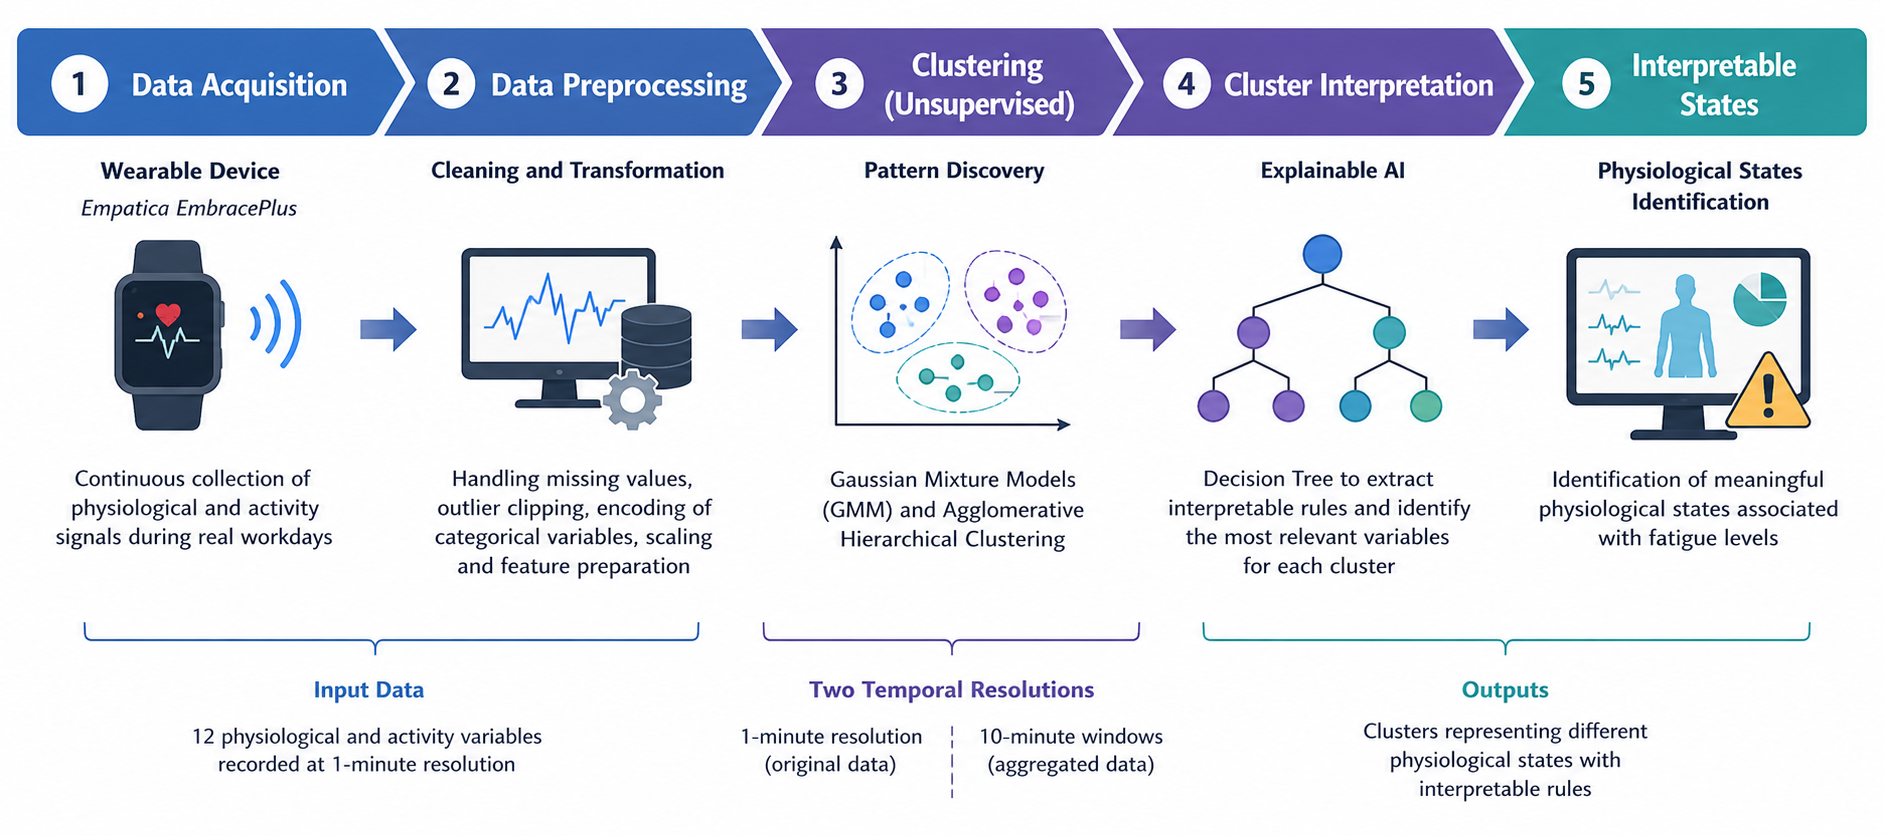
\includegraphics[width=0.9\linewidth]{figs/Figure_1.png}
  \captionof{figure}{Methodological workflow of the study.}
  \label{fig:methodological_workflow}
\end{center}


%%%%%%%%%%%%%%%%%%%%
% RESULTS AND DISCUSSION
%%%%%%%%%%%%%%%%%%%%
\section{Experimental Results and Discussion}\label{sec:results}

This section presents the experimental results obtained from the clustering models developed to identify physiological states using data recorded by the Empatica EmbracePlus device. The experiments were conducted both with the original data, at a one-minute temporal resolution, and with an aggregated representation based on ten-minute temporal windows, to analyze the effect of temporal aggregation on model performance.

First, the training and validation results of the different algorithms are presented, including the metrics used to evaluate clustering quality and the process of selecting the number of clusters. Subsequently, the physiological interpretation of the identified states is presented, followed by a comparative discussion of the models to determine the most suitable approach for identifying physiological states associated with fatigue.

\subsection{Model Performance}

To evaluate the performance of the clustering models and the quality of the identified structures, the configurations obtained with the Gaussian Mixture Model (GMM) and Agglomerative Hierarchical Clustering were analyzed, both with the original data and with data aggregated into 10-minute temporal windows. For the GMM, the Bayesian Information Criterion (BIC) was used as the primary criterion for selecting the model structure. For Agglomerative Hierarchical Clustering, the Silhouette score, complemented by the elbow curve, was used to support the selection of the optimal number of clusters.

\begin{center}
\captionof{table}{Structural Metrics of the Clustering Models}
\label{tab:clustering_metrics}
\resizebox{\textwidth}{!}{%
\begin{tabular}{l c c c c c}
\hline
Algorithm & Data & Original / PCA & Selection Criterion & Clusters ($k$) & Silhouette Score \\
\hline
GMM & Original & 12 / 6 & BIC & 9 & 0.3475 \\
GMM & Windows (10 min) & 12 / 4 & BIC & 5 & 0.3742 \\
\hline
Hierarchical Clustering & Original & 12 / -- & Silhouette + Elbow & 5 & 0.3959 \\
Hierarchical Clustering & Windows (10 min) & 12 / -- & Silhouette + Elbow & 5 & 0.4132 \\
\hline
\end{tabular}%
}
\end{center}

\textbf{Table} \ref{tab:clustering_metrics} summarizes the main configurations evaluated. For the \textbf{GMM}, the original data were reduced through \textit{Principal Component Analysis (PCA)}, from 12 to 6 components before training. This transformation reduced the complexity of the feature space while preserving approximately 90\% of the original data variance. In turn, the window-based representation used only 4 components, suggesting that data smoothing simplified its representation and consequently reduced the number of parameters to be estimated, favoring greater stability during learning. In contrast, \textbf{Agglomerative Hierarchical Clustering} was applied directly to the normalized variables, without dimensionality reduction through PCA. The results show that using 10-minute temporal windows improved the \textit{Silhouette} score for both algorithms. For the GMM, the value increased from 0.3475 to 0.3742, whereas for Hierarchical Clustering it increased from 0.3959 to 0.4132. These results indicate that temporal aggregation favored the formation of clusters with greater internal cohesion and better separation between groups.

In comparative terms, Hierarchical Clustering presented the highest Silhouette values for both temporal representations. However, performance evaluation was not limited exclusively to this metric, since a solution with higher geometric quality may produce an excessive number of clusters or be difficult to interpret from a physiological perspective. For this reason, the final configuration was selected by jointly considering quality metrics, cluster structure, and physiological interpretability.

\subsection{Selection of the Number of Clusters}

Selecting the number of clusters is a fundamental aspect of the clustering process, since it determines the level of detail with which the different physiological states are represented. For the GMM, this selection was performed mainly using the Bayesian Information Criterion (BIC), whereas for Hierarchical Clustering the Silhouette score, the elbow method (\textit{Elbow Method}), and the dendrogram were considered jointly.

For the GMM applied to the original data at a one-minute temporal resolution, the BIC identified a nine-cluster solution as the configuration with the best fit according to this criterion. However, this solution showed substantial fragmentation of the physiological states, making direct interpretation difficult.

For data aggregated into 10-minute temporal windows, the GMM selected five clusters according to the BIC, reaching a Silhouette value of 0.3742. This configuration provided a more favorable balance between structural quality and cluster interpretability. As illustrated in Figure \ref{fig:bic_curves}, the original data show a decreasing BIC trend leading to the selection of nine clusters, whereas the 10-minute window data produce a more defined structure around five clusters.

\begin{center}
  \begin{minipage}{0.48\textwidth}
    \centering
    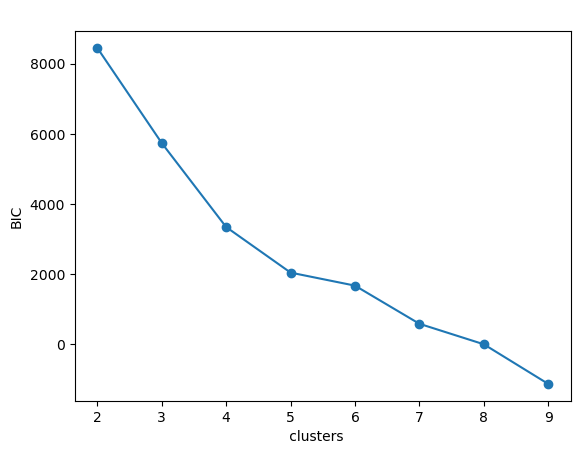
\includegraphics[width=\textwidth]{figs/Figure_2a.png}
    \centerline{(a) Original Data (one-minute resolution)}
  \end{minipage}
  \hfill
  \begin{minipage}{0.48\textwidth}
    \centering
    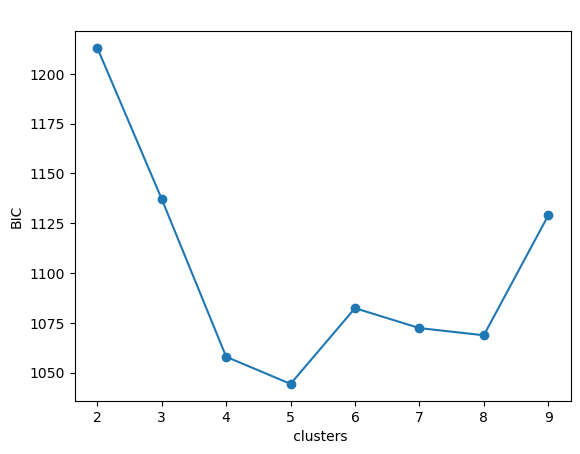
\includegraphics[width=\textwidth]{figs/Figure_2b.png}
    \centerline{(b) 10-Minute Windows}
  \end{minipage}
  \captionof{figure}{Bayesian Information Criterion (BIC) curves obtained for the GMM.}
  \label{fig:bic_curves}
\end{center}

For Agglomerative Hierarchical Clustering, the final configuration was selected through a joint analysis of the Silhouette score, the elbow method (\textit{Elbow Method}), and the dendrograms obtained for the two temporal representations. Although the individual metrics identified different solutions as optimal from a strictly geometric perspective, selecting five clusters provided a balance between cluster quality, segmentation detail, and interpretability of the identified physiological states.

Figures \ref{fig:elbow_curves}(a) and \ref{fig:elbow_curves}(b) show the elbow-method curves for the original data, with a one-minute temporal resolution, and for the data aggregated into 10-minute windows, respectively. These curves represent the evolution of the Within-Cluster Sum of Squares (WCSS) as a function of the number of clusters. Although WCSS decreases as $k$ increases, the goal is to identify the point beyond which adding new clusters provides progressively smaller improvements. In both cases, a sharp reduction is observed for low values of $k$, followed by a more gradual decrease. The windowed data exhibit lower WCSS values, consistently with the lower variability introduced by temporal aggregation. Although neither curve presents a clearly defined elbow point, both reveal a stabilization trend for intermediate solutions, discouraging excessively fragmented segmentation.

\begin{center}
  \begin{minipage}{0.48\textwidth}
    \centering
    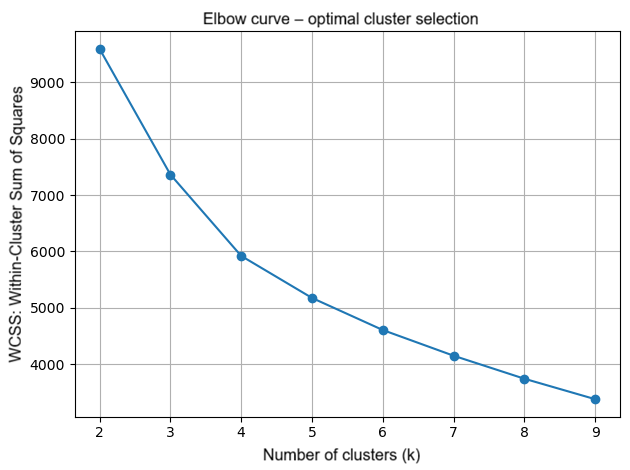
\includegraphics[width=\textwidth]{figs/Figure_3a.png}
    \centerline{(a) Elbow Curve (raw 1-min data)}
  \end{minipage}
  \hfill
  \begin{minipage}{0.48\textwidth}
    \centering
    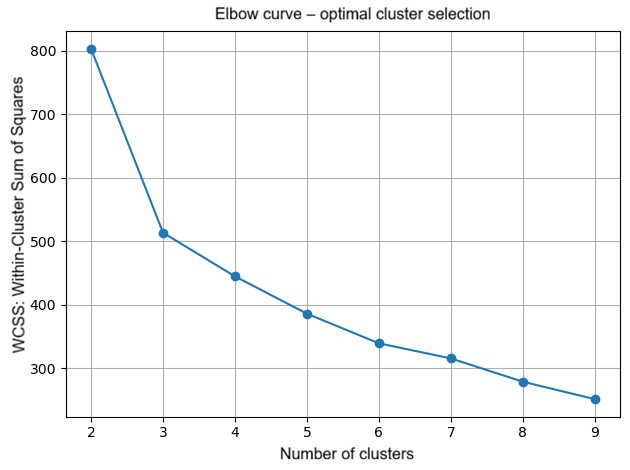
\includegraphics[width=\textwidth]{figs/Figure_3b.png}
    \centerline{(b) Elbow Curve (smoothed 10-min data)}
  \end{minipage}
  \captionof{figure}{Elbow-method curves for Agglomerative Hierarchical Clustering.}  \label{fig:elbow_curves}
\end{center}

The curves presented in Figures \ref{fig:silhouette_curves}(a) and \ref{fig:silhouette_curves}(b) show the evolution of the \textbf{Silhouette} score for different values of $k$. For the original data, the maximum value is obtained for $k=8$. However, from approximately five clusters onward, a relatively stable region is observed, in which score variations are small until this maximum is reached. This result indicates that the intermediate solutions have comparable geometric quality. Thus, selecting $k=8$ does not necessarily imply a sufficiently significant improvement to justify greater fragmentation of the physiological states. For the data aggregated into 10-minute windows, the maximum \textit{Silhouette} score is obtained for $k=2$. Although this configuration provides the best geometric separation according to this metric, a division into only two groups is too general to represent the diversity of physiological behaviors observed over a complete workday. For $k=5$, the score remains competitive and allows a more detailed representation of the different states. Consequently, the analysis of the \textit{Silhouette} score demonstrates that selecting $k$ should not rely exclusively on the maximum metric value, but should also consider the usefulness of the resulting segmentation and the identification of possible inflection points or changes in the score trend.

\begin{center}
  \begin{minipage}{0.48\textwidth}
    \centering
    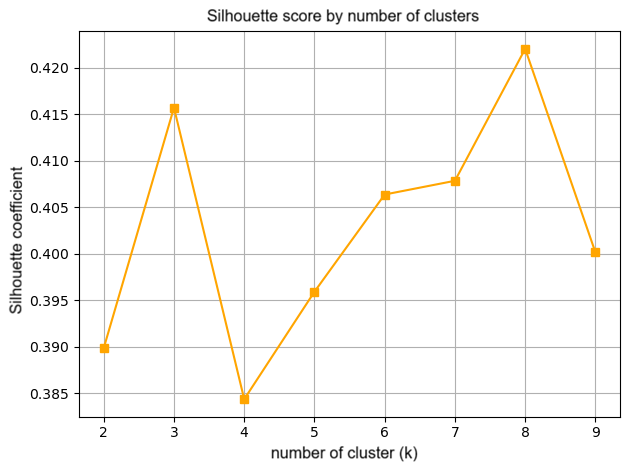
\includegraphics[width=\textwidth]{figs/Figure_4a.png}
    \centerline{(a) Original data (1 minute)}
  \end{minipage}
  \hfill
  \begin{minipage}{0.48\textwidth}
    \centering
    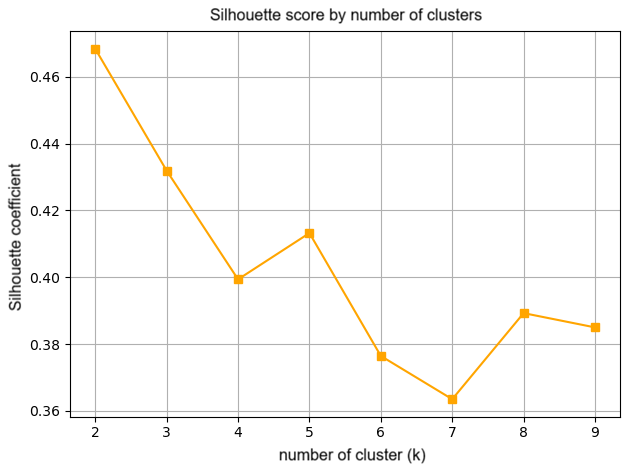
\includegraphics[width=\textwidth]{figs/Figure_4b.png}
    \centerline{(b) Aggregated data (10 minutes)}
  \end{minipage}
  \captionof{figure}{Evolution of the \textit{Silhouette} score for different values of $k$.}  \label{fig:silhouette_curves}
\end{center}

Figures \ref{fig:dendrogram_original} and \ref{fig:dendrogram_window} show the \textbf{dendrograms} corresponding to the original data and the data aggregated into 10-minute windows, respectively. This representation makes it possible to observe the hierarchical structure of the data and analyze the distances at which successive merges between groups occur. In the dendrogram corresponding to the original data, merges occur at relatively high distances, reflecting greater dispersion of the observations and, consequently, greater variability in the physiological patterns recorded at the minute level. In contrast, the dendrogram obtained from the temporal windows has a more compact structure, with merges at lower distances, consistent with the smoothing effect produced by temporal aggregation.

In addition to providing information about the hierarchical structure, dendrograms allow different values of $k$ to be evaluated visually by selecting a cut level. For the original data, a cut at approximately distance 100 produces a very general separation into two large groups, whereas a cut near distance 40 produces five distinct clusters. The latter configuration provides sufficiently detailed segmentation without reaching the fragmentation associated with solutions having a large number of clusters. Thus, the dendrogram provides additional visual evidence that complements the results obtained with the elbow method and the \textit{Silhouette} score.

\begin{center}
  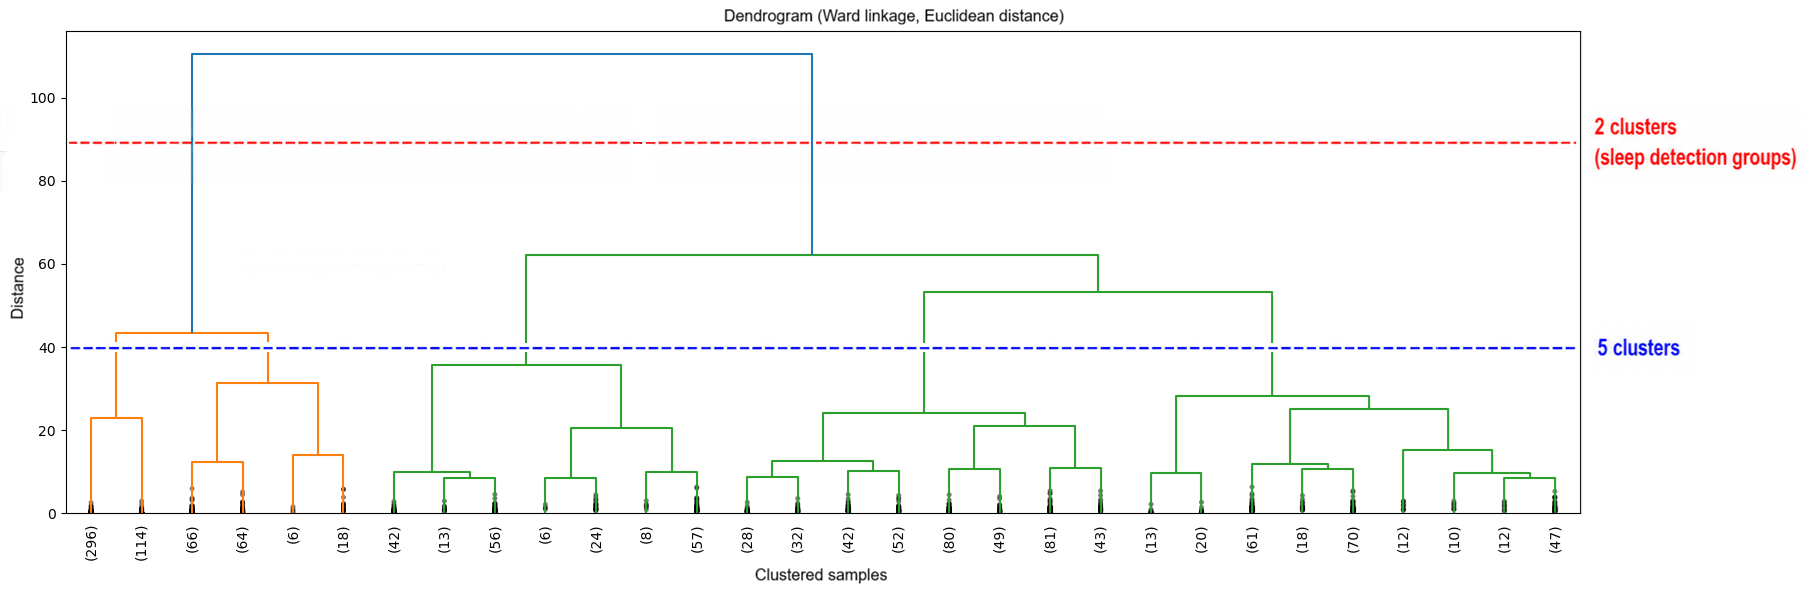
\includegraphics[width=0.95\textwidth]{figs/Figure_5.png}
  \captionof{figure}{Dendrogram of Agglomerative Hierarchical Clustering for the original data.}
  \label{fig:dendrogram_original}
\end{center}

\begin{center}
  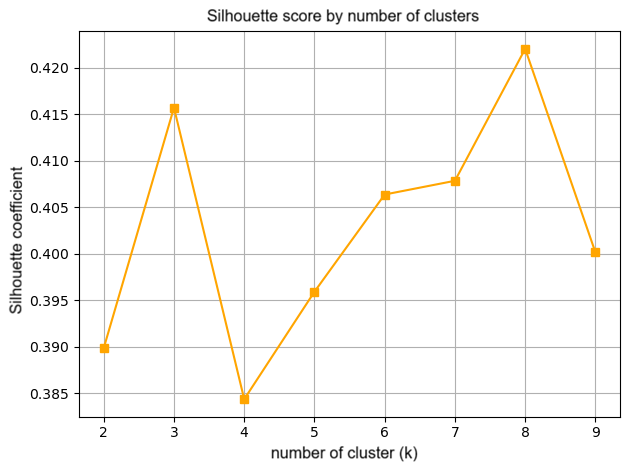
\includegraphics[width=0.95\textwidth]{figs/Figure_6.png}
  \captionof{figure}{Dendrogram of Agglomerative Hierarchical Clustering using 10-minute windows.}
  \label{fig:dendrogram_window}
\end{center}

Taken together, the three criteria provide complementary perspectives on selecting the number of clusters. The \textit{elbow method} identifies the region in which adding new groups no longer produces substantial improvements in internal cohesion; the \textit{Silhouette} score enables comparison of the geometric quality of different partitions; and the \textit{dendrogram} enables visual analysis of the hierarchical structure and separation levels between groups. Considering this evidence jointly and, above all, the need to obtain sufficiently differentiated and interpretable physiological states, a configuration of \textbf{$k=5$ clusters} was finally adopted for Hierarchical Clustering in both temporal representations.


\subsection{Cluster Validation}

To evaluate the consistency and interpretability of the obtained clusters, a Decision Tree was used with the physiological attributes as input variables and the clusters previously identified by Agglomerative Hierarchical Clustering as the target variable. This approach makes it possible to assess the extent to which the clusters can be reproduced through simple decision rules and to identify the variables with the greatest discriminative capacity between the different states. Table \ref{tab:arvore_validacao} presents the results obtained for the original data and for data aggregated into 10-minute temporal windows.

\begin{center}
\captionof{table}{Interpretability Assessment Using a Decision Tree}
\label{tab:arvore_validacao}
\resizebox{\textwidth}{!}{%
\begin{tabular}{l c c c}
\hline
Configuration & Maximum Depth & Training Accuracy & Accuracy (5-Fold CV) \\
\hline
Original Data & 8 & 98.61\% & 92.01\% $\pm$ 4.44\% \\
Windows (10 min) & 5 & 93.06\% & 83.92\% $\pm$ 10.24\% \\
\hline
\end{tabular}%
}
\end{center}

For the original data, the tree achieved an \textit{accuracy} of 98.61\% on the training set and 92.01\% $\pm$ 4.44\% in 5-\textit{fold} cross-validation. For the 10-minute windows, values of 93.06\% in training and 83.92\% $\pm$ 10.24\% in cross-validation were obtained. Although performance was lower after temporal aggregation, the results still indicate that the clusters have sufficiently consistent boundaries to be reproduced by a simple supervised model. This difference should also be interpreted in light of the substantial reduction in the number of observations.

Analysis of the tree structures makes it possible to understand which attributes have the greatest discriminative capacity between clusters. For the original data, with a one-minute temporal resolution, the tree reached a maximum depth of eight levels, reflecting the greater variability and rapid fluctuations of the signals. The most important variables were \texttt{sleep\_detection\_stage} (31.47\%), \texttt{activity\_intensity} (24.54\%), \texttt{walking} (20.88\%), and \texttt{still} (17.06\%). These were followed by \texttt{eda\_scl\_usiemens} (3.25\%), \texttt{step\_counts} (1.90\%), \texttt{pulse\_rate\_bpm} (0.68\%), and \texttt{vector\_magnitude} (0.21\%).

For the representation aggregated into 10-minute windows, the tree had a maximum depth of five levels. In this case, \texttt{still} (41.34\%), \texttt{step\_counts} (29.95\%), and \texttt{walking} (22.85\%) were the most prominent variables, while \texttt{activity\_counts} had an importance of 5.70\% and \texttt{met} made a residual contribution of 0.15\%.

Figure \ref{fig:arvore_jerarquico_original} presents the tree obtained for the original data, whereas Figure \ref{fig:arvore_jerarquico_window} presents the corresponding structure for the 10-minute temporal windows. The extracted rules show that, at the one-minute resolution, the distinction between clusters is initially conditioned by sleep stage and activity level, and is subsequently refined by variables related to movement and physiological response. After temporal aggregation, the decision logic depends mainly on more stable behavioral measures, such as remaining still, step count, and walking. The detailed decision rules for the original data and the 10-minute windows are presented in Tables \ref{tab:regras_originais} and \ref{tab:regras_janelas}, respectively.

\begin{center}
  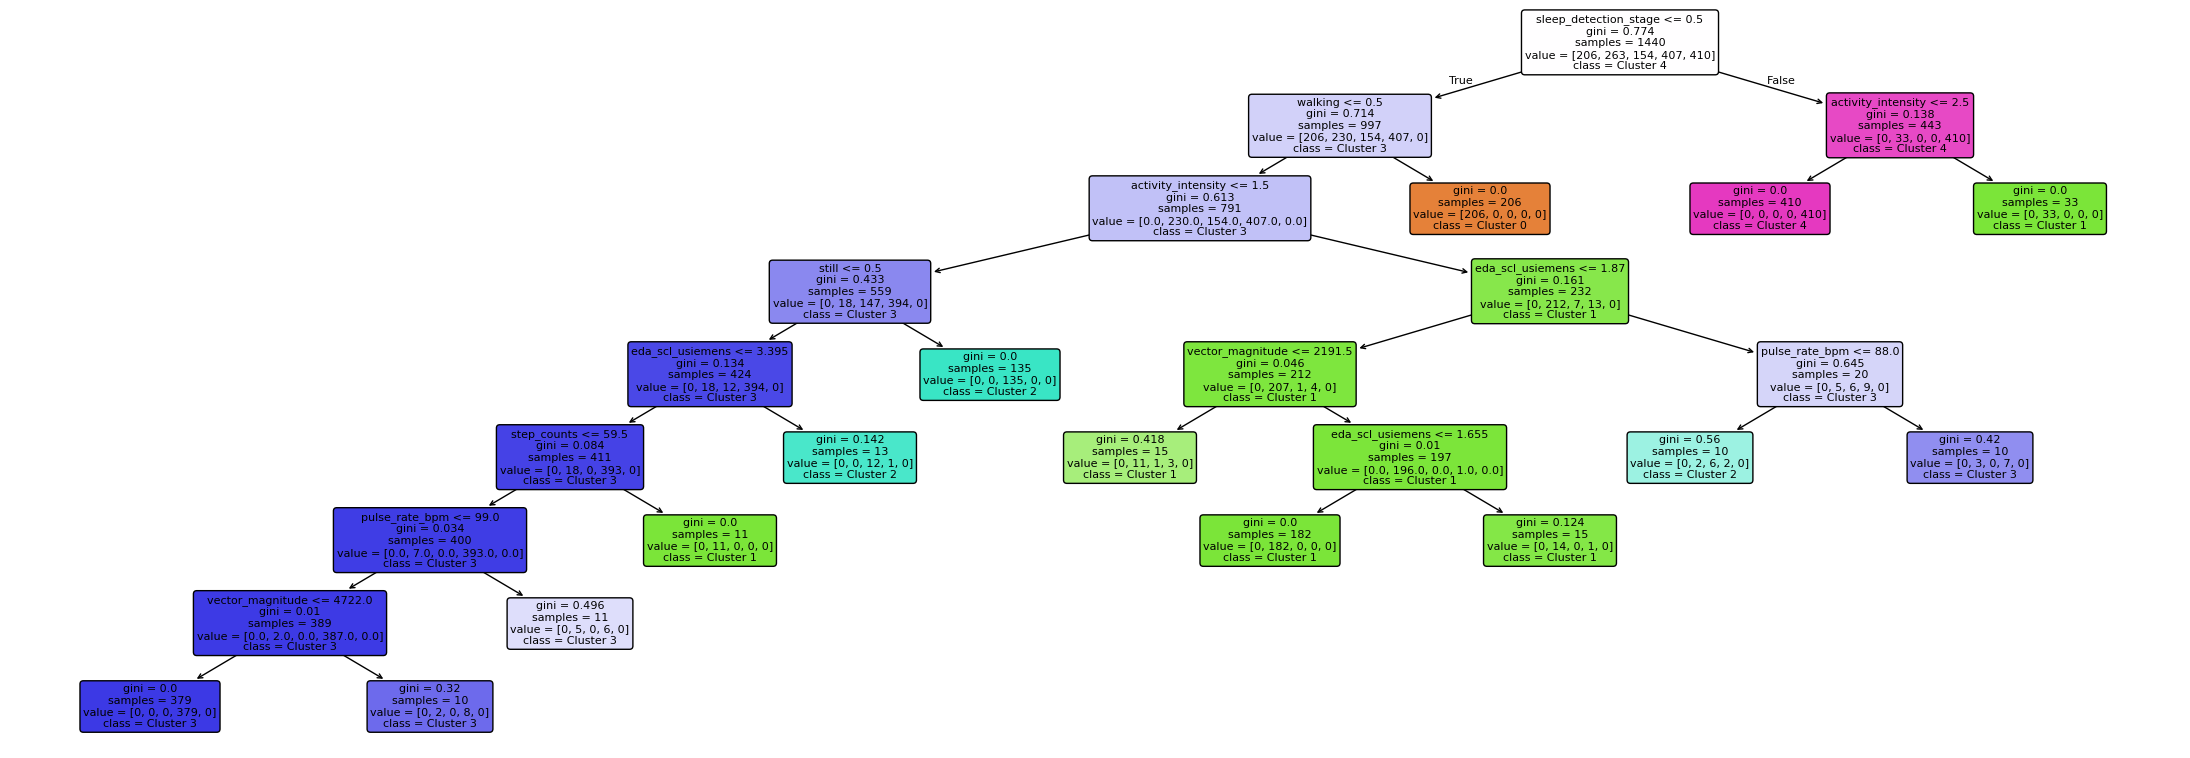
\includegraphics[width=0.95\textwidth]{figs/Figure_7.png}
  \captionof{figure}{Decision Tree for data with one-minute resolution.}
  \label{fig:arvore_jerarquico_original}
\end{center}
\medskip

\begin{center}
  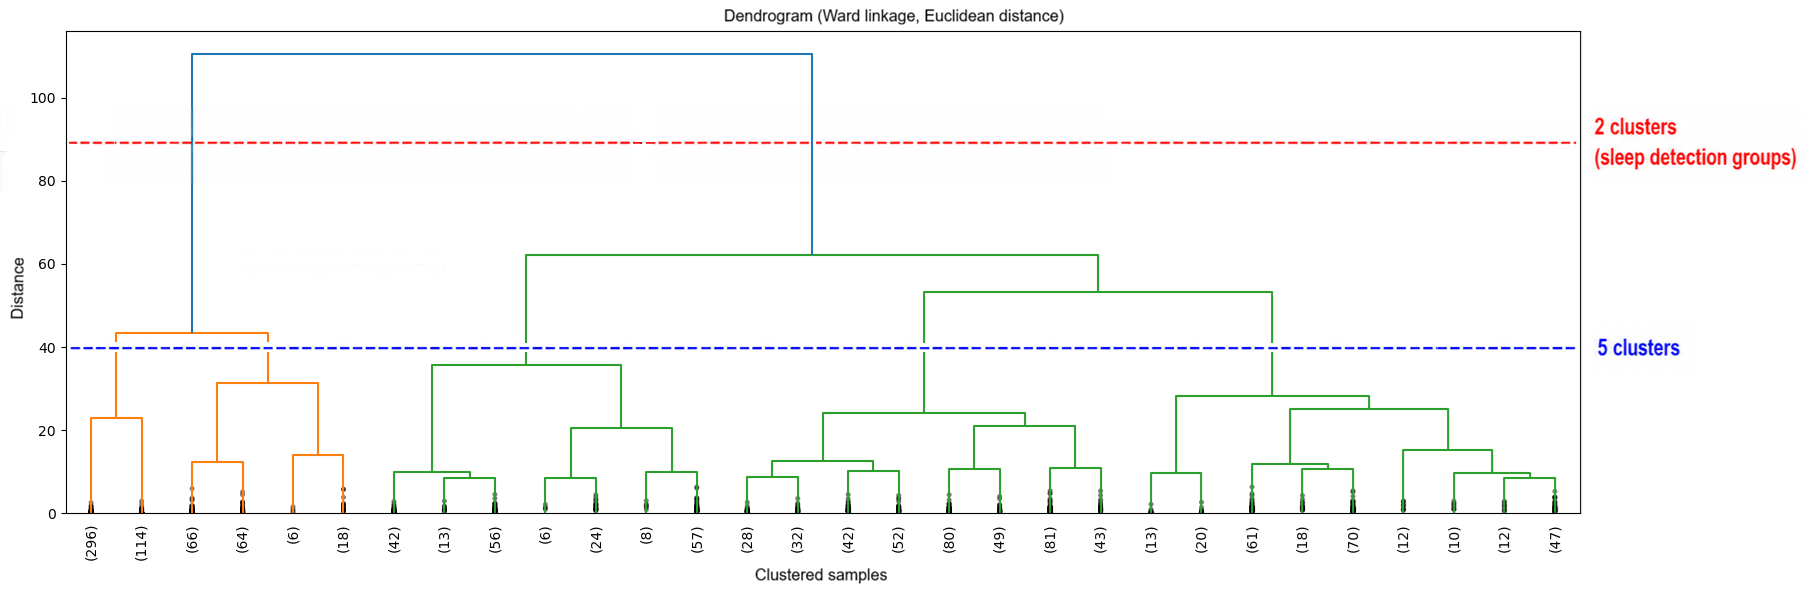
\includegraphics[width=0.95\textwidth]{figs/Figure_8.png}
  \captionof{figure}{Decision Tree for data aggregated into 10-minute windows.}
  \label{fig:arvore_jerarquico_window}
\end{center}
\medskip

\begin{center}
\centering
\captionof{table}{Decision Rules for Cluster Identification (Original Data).}
\label{tab:regras_originais}
\resizebox{\textwidth}{!}{%
\begin{tabular}{l}
\hline
\textbf{Extracted Logical Rules (Temporal Resolution: 1 minute)} \\
\hline
If \textbf{\texttt{sleep\_detection\_stage}} $\le 0.50$: \\
~~If \textbf{\texttt{walking}} $\le 0.50$: \\
~~~~If \textbf{\texttt{activity\_intensity}} $\le 1.50$: \\
~~~~~~If \textbf{\texttt{still}} $\le 0.50$: \\
~~~~~~~~If \textbf{\texttt{eda\_scl\_usiemens}} $\le 3.39$: \\
~~~~~~~~~~If \textbf{\texttt{step\_counts}} $\le 59.50$: \\
~~~~~~~~~~~~If \textbf{\texttt{pulse\_rate\_bpm}} $\le 99.00$: \\
~~~~~~~~~~~~~~If \textbf{\texttt{vector\_magnitude}} $\le 4722.00 \rightarrow$ \textbf{Cluster 3} (Transitional/low-movement activity) \\
~~~~~~~~~~~~~~If \textbf{\texttt{vector\_magnitude}} $> 4722.00 \rightarrow$ \textbf{Cluster 3} (Residual physical activity at rest) \\
~~~~~~~~~~~~~~If \textbf{\texttt{pulse\_rate\_bpm}} $> 99.00 \rightarrow$ \textbf{Cluster 3} (Brief physiological activation without locomotion) \\
~~~~~~~~~~If \textbf{\texttt{step\_counts}} $> 59.50 \rightarrow$ \textbf{Cluster 1} (Brief transitional movement) \\
~~~~~~~~If \textbf{\texttt{eda\_scl\_usiemens}} $> 3.39 \rightarrow$ \textbf{Cluster 2} (Static work with high sympathetic reactivity) \\
~~~~~~If \textbf{\texttt{still}} $> 0.50 \rightarrow$ \textbf{Cluster 2} (Typical sedentary/static work) \\
~~~~If \textbf{\texttt{activity\_intensity}} $> 1.50$: \\
~~~~~~If \textbf{\texttt{eda\_scl\_usiemens}} $\le 1.87 \rightarrow$ \textbf{Cluster 1} (Light physical effort with low electrodermal conductance) \\
~~~~~~If \textbf{\texttt{eda\_scl\_usiemens}} $> 1.87 \rightarrow$ \textbf{Cluster 3} (Moderate physical effort with greater sympathetic activation) \\
~~If \textbf{\texttt{walking}} $> 0.50 \rightarrow$ \textbf{Cluster 0} (Walking-related physical activity) \\
If \textbf{\texttt{sleep\_detection\_stage}} $> 0.50$: \\
~~If \textbf{\texttt{activity\_intensity}} $\le 2.50 \rightarrow$ \textbf{Cluster 4} (Rest or deep-sleep phase with low activation) \\
~~If \textbf{\texttt{activity\_intensity}} $> 2.50 \rightarrow$ \textbf{Cluster 1} (Rest phase with light-movement transitions) \\
\hline
\end{tabular}%
}
\end{center}

\begin{center}
\centering
\captionof{table}{Decision Rules for Cluster Identification (10-Minute Windows).}
\label{tab:regras_janelas}
\resizebox{\textwidth}{!}{%
\begin{tabular}{l}
\hline
\textbf{Extracted Logical Rules (Temporal Aggregation: 10-Minute Windows)} \\
\hline
If \textbf{\texttt{still}} $\le 0.85$: \\
~~If \textbf{\texttt{step\_counts}} $\le 6.45$: \\
~~~~If \textbf{\texttt{walking}} $\le 0.05$ $\rightarrow$ \textbf{Cluster 0} (Brief sedentary-movement transitions) \\
~~~~If \textbf{\texttt{walking}} $> 0.05$ $\rightarrow$ \textbf{Cluster 0} (Brief transitions involving very light walking) \\
~~If \textbf{\texttt{step\_counts}} $> 6.45$: \\
~~~~If \textbf{\texttt{walking}} $\le 0.45$: \\
~~~~~~If \textbf{\texttt{activity\_counts}} $\le 79.65$ $\rightarrow$ \textbf{Cluster 4} (Work with generalized movement at a calm pace) \\
~~~~~~If \textbf{\texttt{activity\_counts}} $> 79.65$: \\
~~~~~~~~If \textbf{\texttt{met}} $\le 2.69$ $\rightarrow$ \textbf{Cluster 2} (Light physical work with controlled metabolic load) \\
~~~~~~~~If \textbf{\texttt{met}} $> 2.69$ $\rightarrow$ \textbf{Cluster 2} (Active work involving varied movement) \\
~~~~If \textbf{\texttt{walking}} $> 0.45$ $\rightarrow$ \textbf{Cluster 3} (Continuous or prolonged active walking) \\
If \textbf{\texttt{still}} $> 0.85$ $\rightarrow$ \textbf{Cluster 1} (Dominant static state: consolidated rest or stable sleep) \\
\hline
\end{tabular}%
}
\end{center}

Taken together, cluster validation confirmed the consistency of the obtained solutions and, for \textbf{Agglomerative Hierarchical Clustering}, also enabled a more interpretable representation of the identified states. Through \textbf{Decision Trees}, the assignments generated by the hierarchical model, whose clustering logic is not directly interpretable, could be transformed into a set of rules based on physiological-variable thresholds, with behavior close to that of heuristic rules. This transformation is particularly relevant because it explicitly identifies the conditions associated with each state and facilitates the interpretation and subsequent application of the \textit{clustering} results.


\subsection{Interpretation of the Physiological Clusters}

An essential step in this investigation was interpreting the clusters generated by the different clustering models, with the aim of understanding the meaning of each group and verifying whether they corresponded to real physiological and behavioral states. For this purpose, the relative levels of the physiological and behavioral variables (\textit{LOW}, \textit{MED}, and \textit{HIGH}) were analyzed together with the distribution of the clusters throughout the workday. This analysis made it possible to relate the different clusters to states such as rest, wakefulness, physical activity, and cognitive load, while also verifying whether their occurrence over time was consistent with these states.

\subsubsection{GMM with Original Data ($k=9$)}

The physiological interpretation of the clusters obtained by the \textit{Gaussian Mixture Model} (GMM) using the original data at the minute level was based on the relative signature of the physiological and behavioral variables and the temporal distribution of the clusters throughout the day. Table \ref{tab:percentis_gmm_original} presents the relative \textit{LOW}, \textit{MED}, and \textit{HIGH} values of the main variables, enabling characterization of the different states identified by the model.

\begin{center}
  \captionof{table}{Physiological signature of the GMM clusters using original data ($k=9$, one-minute resolution).}
    \label{tab:percentis_gmm_original}
    \renewcommand{\arraystretch}{1.4}
    \resizebox{\textwidth}{!}{%
    \begin{tabular}{c c c c c c c c c c}
    \hline
    \textbf{Cluster} & \textbf{EDA} & \textbf{Pulse Rate} & \textbf{MET} & \textbf{Act. Counts} & \textbf{Step Counts} & \textbf{Vec. Mag.} & \textbf{Act. Intensity} & \textbf{Sleep Stage} & \textbf{Proposed Physiological Meaning} \\
    \hline
    5 & \textit{LOW} & \textit{MED} & \textit{LOW} & \textit{LOW} & \textit{LOW} & \textit{LOW} & \textit{LOW} & \textit{HIGH} & [Sleep group] onset \\
    0 & \textit{MED} & \textit{LOW} & \textit{LOW} & \textit{LOW} & \textit{LOW} & \textit{LOW} & \textit{LOW} & \textit{HIGH} & [Sleep group] deep sleep \\
    1 & \textit{LOW} & \textit{MED} & \textit{HIGH} & \textit{MED} & \textit{HIGH} & \textit{HIGH} & \textit{HIGH} & \textit{HIGH} & [Wakefulness group] \\
    7 & \textit{HIGH} & \textit{MED} & \textit{MED} & \textit{LOW} & \textit{MED} & \textit{MED} & \textit{MED} & \textit{HIGH} & [Sedentary/focus group] baseline state \\
    2 & \textit{HIGH} & \textit{MED} & \textit{MED} & \textit{MED} & \textit{MED} & \textit{MED} & \textit{MED} & \textit{LOW} & [Sedentary/focus group] work/concentration \\
    6 & \textit{HIGH} & \textit{LOW} & \textit{MED} & \textit{MED} & \textit{MED} & \textit{MED} & \textit{MED} & \textit{LOW} & [Sedentary/focus group] stress peak \\
    3 & \textit{LOW} & \textit{HIGH} & \textit{HIGH} & \textit{HIGH} & \textit{HIGH} & \textit{HIGH} & \textit{HIGH} & \textit{LOW} & [Physical-activity group] walking \\
    8 & \textit{LOW} & \textit{MED} & \textit{HIGH} & \textit{HIGH} & \textit{HIGH} & \textit{HIGH} & \textit{HIGH} & \textit{LOW} & [Physical-activity group] general movement \\
    4 & \textit{HIGH} & \textit{HIGH} & \textit{HIGH} & \textit{HIGH} & \textit{HIGH} & \textit{HIGH} & \textit{HIGH} & \textit{LOW} & [Physical-activity group] intense activity \\
    \hline
    \end{tabular}%
    }
\end{center}

The analysis of Table \ref{tab:percentis_gmm_original} shows that, although the nine clusters correspond to the statistically optimal solution according to the BIC, several have similar physiological signatures, differing mainly in activity intensity or physiological activation level. The clusters can therefore be interpreted as different manifestations of four main functional states: rest/sleep, wakefulness, sedentary behavior or concentration, and physical activity. The sleep-related clusters show low levels of movement and energy expenditure, whereas the physical-activity groups show high MET, step, movement, and activity-intensity values. Between these extremes, the sedentary and concentration-related clusters are distinguished mainly by increased EDA and moderate activity levels.

The temporal distribution presented in Figure \ref{fig:temporal_gmm_original} complements this characterization by showing how the different clusters succeed one another over 24 hours.

\begin{center}
  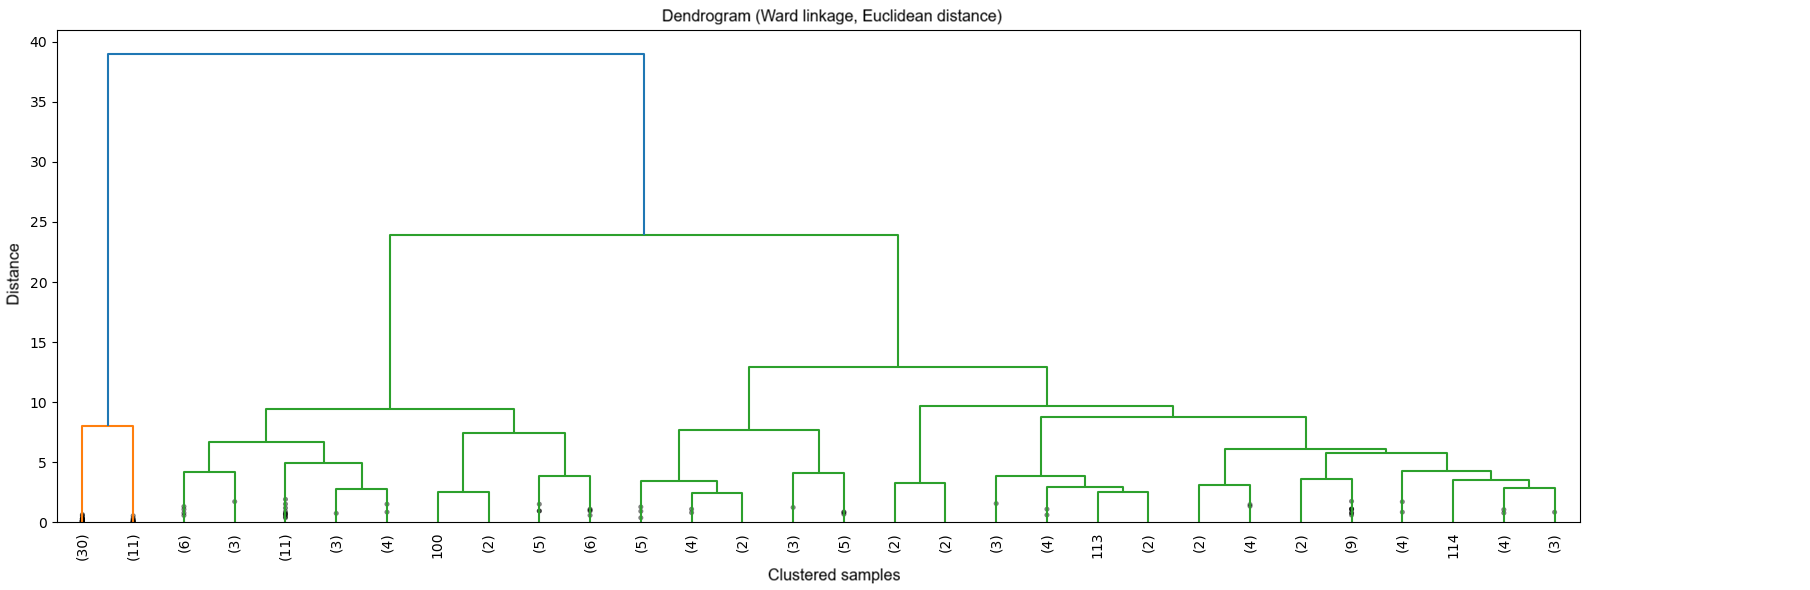
\includegraphics[width=0.95\textwidth]{figs/Figure_9.png}
  \captionof{figure}{Daily temporal distribution of the GMM clusters using one-minute data.}
    \label{fig:temporal_gmm_original}
\end{center}

Despite the high level of detail provided by the minute-level data, greater alternation between states and more fragmented segmentation are observed. Thus, the nine clusters do not necessarily represent nine distinct physiological states, but may correspond to different variations of a smaller set of functional states. This interpretation is important for the subsequent analysis because it makes it possible to relate the clusters identified by the GMM to physiological and behavioral states observable throughout the daily routine.


\subsubsection{GMM with 10-Minute Windows ($k=5$)}

For data aggregated into 10-minute windows, the GMM was configured with five clusters, providing a more compact representation of the physiological states. Table \ref{tab:percentis_gmm_janela} presents the relative cluster signature.

\begin{center}
  \captionof{table}{Physiological signature of the GMM clusters ($k=5$, 10-minute windows).}
    \label{tab:percentis_gmm_janela}
    \renewcommand{\arraystretch}{1.4}
    \resizebox{\textwidth}{!}{%
    \begin{tabular}{c c c c c c c c c c}
    \textbf{Cluster} & \textbf{EDA} & \textbf{Pulse Rate} & \textbf{MET} & \textbf{Act. Counts} & \textbf{Step Counts} & \textbf{Vec. Mag.} & \textbf{Act. Intensity} & \textbf{Sleep Stage} & \textbf{Proposed Physiological Meaning} \\
    \hline
    0 & \textit{LOW} & \textit{LOW} & \textit{HIGH} & \textit{MED} & \textit{HIGH} & \textit{MED} & \textit{HIGH} & \textit{HIGH} & Getting Out of Bed / Morning Transition \\
    1 & \textit{MED} & \textit{LOW} & \textit{LOW} & \textit{LOW} & \textit{LOW} & \textit{LOW} & \textit{LOW} & \textit{HIGH} & Stable Sleep / Rest State \\
    2 & \textit{HIGH} & \textit{HIGH} & \textit{HIGH} & \textit{HIGH} & \textit{HIGH} & \textit{HIGH} & \textit{HIGH} & \textit{LOW} & Peaks of Physical Intensity \\
    3 & \textit{HIGH} & \textit{MED} & \textit{MED} & \textit{MED} & \textit{MED} & \textit{MED} & \textit{MED} & \textit{HIGH} & Workday / Cognitive Load \\
    4 & \textit{LOW} & \textit{MED} & \textit{HIGH} & \textit{HIGH} & \textit{HIGH} & \textit{HIGH} & \textit{HIGH} & \textit{HIGH} & Active Routine and Travel \\
    \hline
    \end{tabular}%
    }
\end{center}

The five clusters have distinct physiological signatures and identify states associated with rest, the transition between sleep and wakefulness, daily activity, cognitive load, and periods of greater physical intensity. The \textit{Stable Sleep} cluster is characterized by low activity, heart-rate, and energy-expenditure levels, whereas the \textit{Morning Transition} cluster combines high MET and movement levels with still-low heart-rate and EDA values. The \textit{Active Routine and Travel} cluster shows high movement and activity indicators, consistent with travel and light physical activity. In turn, \textit{Workday / Cognitive Load} is distinguished mainly by high EDA and moderate activity, whereas \textit{Peaks of Physical Intensity} show high values for most variables, corresponding to episodes of greatest physical demand.

The temporal distribution of these clusters throughout the workday is presented in Figure \ref{fig:temporal_gmm_janela}.

\begin{center}
  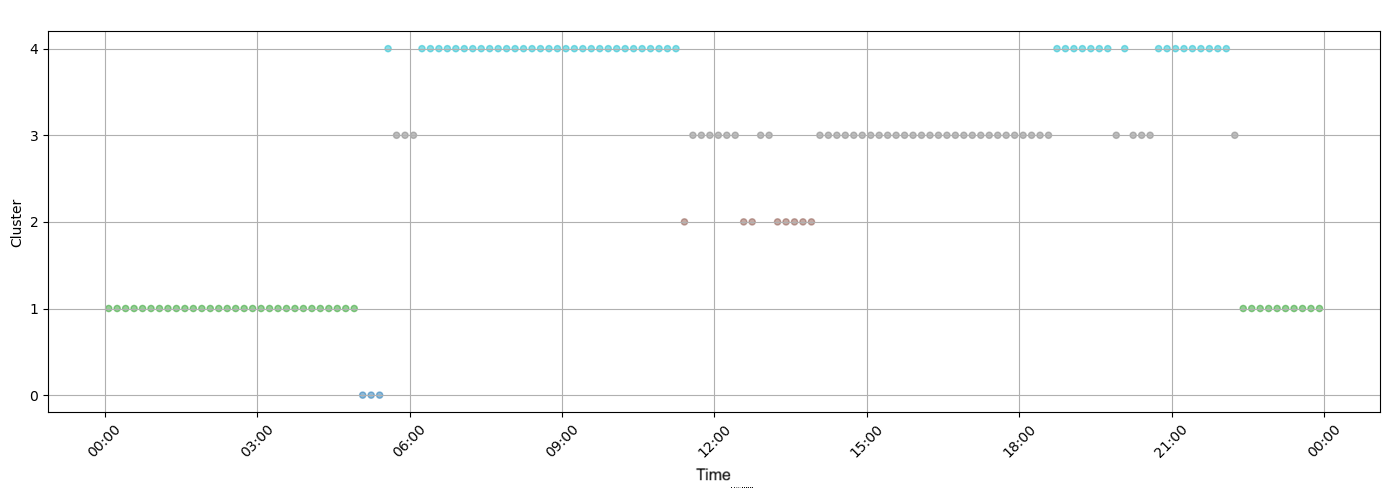
\includegraphics[width=0.95\textwidth]{figs/Figure_10.png}
  \captionof{figure}{Daily temporal distribution of the GMM clusters ($k=5$, 10-minute windows) throughout a workday.}
    \label{fig:temporal_gmm_janela}
\end{center}

The temporal distribution shows a more stable organization of the physiological states, with relatively continuous periods of rest, daily activity, and work-related load. In particular, a coherent sequence is observed between the sleep period, the morning transition, activities and travel, the workday, and occasional episodes of greater intensity. This organization contrasts with the greater fragmentation observed in the minute-level data and suggests that temporal aggregation reduces instantaneous signal fluctuations, facilitating the identification of more stable and interpretable physiological states.


\subsubsection{Hierarchical Clustering with Original Data ($k=5$)}

For \textit{Agglomerative Hierarchical Clustering} applied to the original data at the minute level, a five-cluster configuration was adopted. The physiological characterization of the obtained clusters is presented in Table \ref{tab:percentis_hier_original}, considering the relative levels of the physiological and behavioral variables.

\begin{center}
\captionof{table}{Physiological Signature of the Hierarchical Clustering Clusters ($k=5$, Minute-Level Data)}
\label{tab:percentis_hier_original}
\renewcommand{\arraystretch}{1.4}
\resizebox{\textwidth}{!}{%
\begin{tabular}{c c c c c c c c c c}
\hline
\textbf{Cluster} & \textbf{EDA} & \textbf{Pulse Rate} & \textbf{MET} & \textbf{Act. Counts} & \textbf{Step Counts} & \textbf{Vec. Mag.} & \textbf{Act. Intensity} & \textbf{Sleep Stage} & \textbf{Proposed Physiological Meaning} \\
\hline
0 & \textit{MED} & \textit{HIGH} & \textit{HIGH} & \textit{HIGH} & \textit{HIGH} & \textit{HIGH} & \textit{HIGH} & \textit{LOW} & Active Movement and Walking \\
1 & \textit{MED} & \textit{MED} & \textit{HIGH} & \textit{HIGH} & \textit{HIGH} & \textit{HIGH} & \textit{HIGH} & \textit{HIGH} & Activity with Sleep Presence \\
2 & \textit{HIGH} & \textit{MED} & \textit{MED} & \textit{MED} & \textit{MED} & \textit{MED} & \textit{MED} & \textit{LOW} & Concentration / Cognitive Load \\
3 & \textit{HIGH} & \textit{MED} & \textit{MED} & \textit{HIGH} & \textit{HIGH} & \textit{MED} & \textit{MED} & \textit{LOW} & Physical Effort / Intense Activity \\
4 & \textit{MED} & \textit{LOW} & \textit{MED} & \textit{LOW} & \textit{MED} & \textit{LOW} & \textit{MED} & \textit{HIGH} & Rest or Sleep \\
\hline
\end{tabular}%
}
\end{center}

The signatures make it possible to identify states associated with rest, concentration, and physical activity. The \textit{Rest or Sleep} cluster has the lowest activity and heart-rate levels, together with high \textit{Sleep Stage} values. In contrast, the \textit{Active Movement and Walking} and \textit{Physical Effort / Intense Activity} clusters show high movement and activity levels. The \textit{Concentration / Cognitive Load} cluster is distinguished mainly by high EDA and moderate activity levels. In turn, the \textit{Activity with Sleep Presence} cluster combines high activity levels with a high \textit{Sleep Stage} value, resulting in a less intuitive signature from a physiological perspective.

The temporal distribution of the clusters throughout the workday is presented in Figure \ref{fig:temporal_hier_original}.

\begin{center}
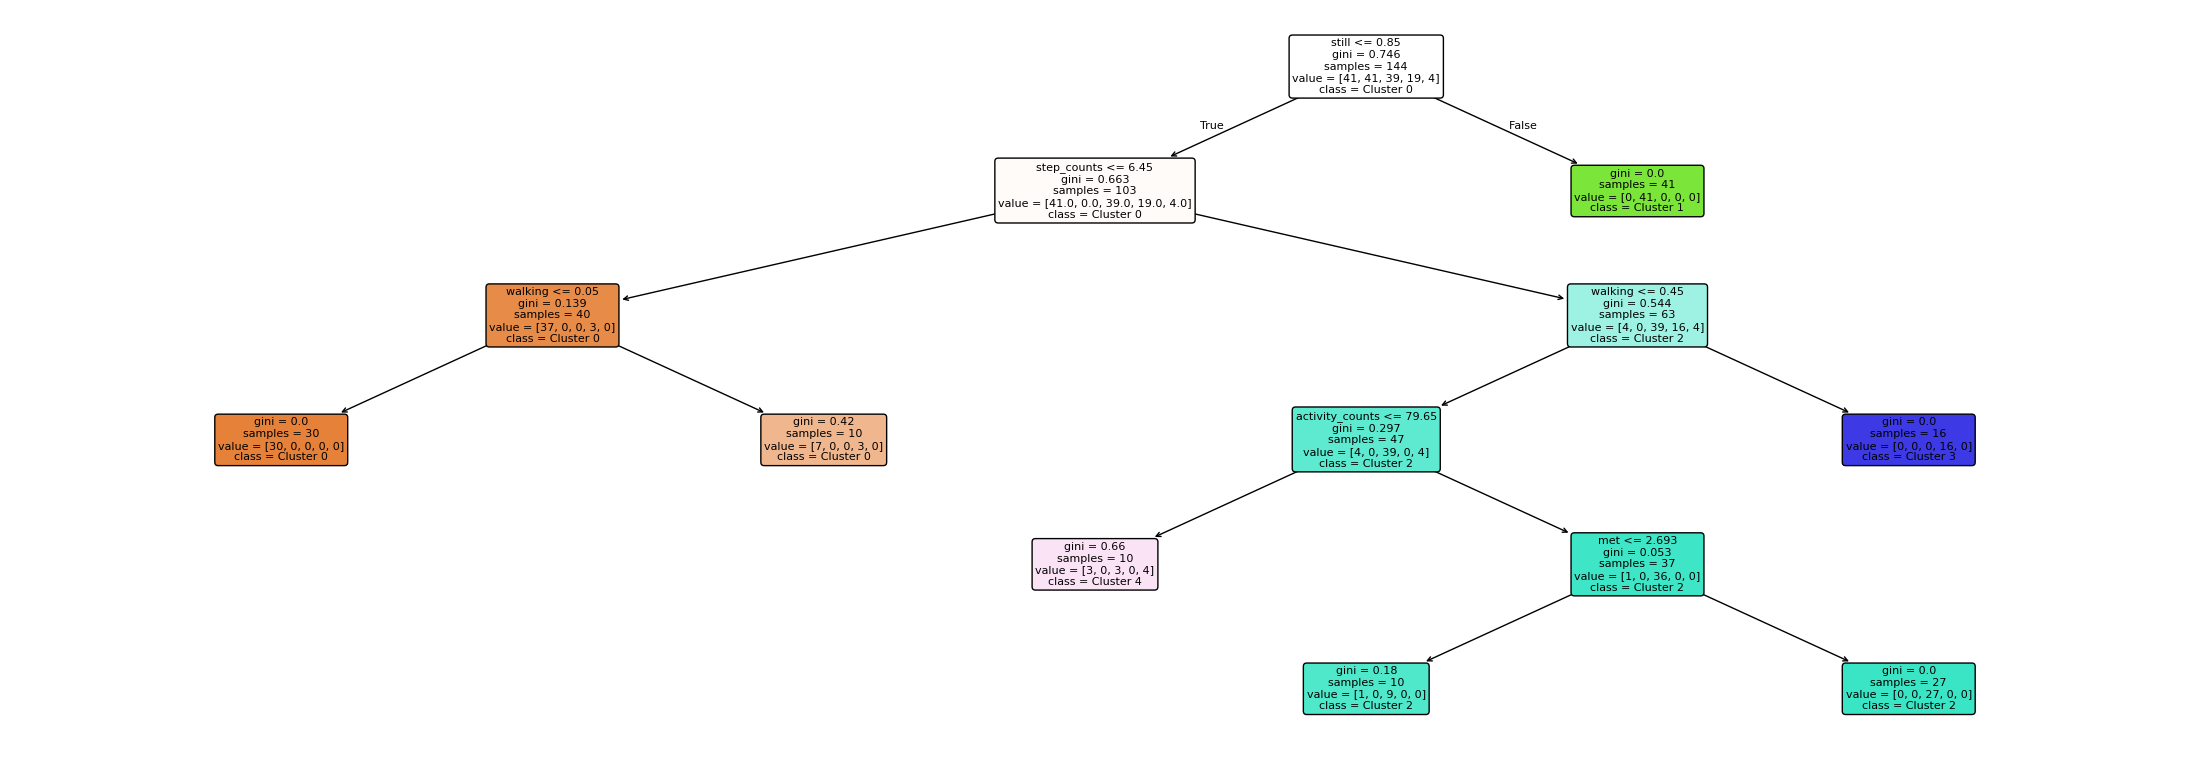
\includegraphics[width=0.95\textwidth]{figs/Figure_11.png}
\captionof{figure}{Daily temporal distribution of the Hierarchical Clustering clusters ($k=5$, minute-level data) throughout a workday.}
\label{fig:temporal_hier_original}
\end{center}

The temporal distribution shows greater alternation between states than the GMM, with more frequent transitions and less continuous evolution throughout the day. Although the \textit{Rest or Sleep} and \textit{Concentration / Cognitive Load} clusters occur at times compatible with rest and work-related activity, respectively, the remaining clusters are more dispersed. Thus, although the model distinguishes different levels of activity and physiological load, greater temporal variability and overlap between some signatures reduce the consistency of the physiological interpretation compared with that obtained using the GMM.


\subsubsection{Hierarchical Clustering with 10-Minute Windows ($k=5$)}

For data aggregated into 10-minute windows, \textit{Agglomerative Hierarchical Clustering} was configured with five clusters. Table \ref{tab:percentis_hier_janela} presents the relative signature of the obtained clusters, enabling identification of physiological states associated with rest, awakening, daily activity, cognitive load, and physical effort.

\begin{center}
\captionof{table}{Physiological Signature of the Hierarchical Clustering Clusters ($k=5$, 10-Minute Windows)}
\label{tab:percentis_hier_janela}
\renewcommand{\arraystretch}{1.4}
\resizebox{\textwidth}{!}{%
\begin{tabular}{c c c c c c c c c c}
\hline
\textbf{Cluster} & \textbf{EDA} & \textbf{Pulse Rate} & \textbf{MET} & \textbf{Act. Counts} & \textbf{Step Counts} & \textbf{Vec. Mag.} & \textbf{Act. Intensity} & \textbf{Sleep Stage} & \textbf{Proposed Physiological Meaning} \\
\hline
0 & \textit{HIGH} & \textit{MED} & \textit{MED} & \textit{MED} & \textit{MED} & \textit{MED} & \textit{MED} & \textit{LOW} & Concentration and Work / Main Workday \\
1 & \textit{MED} & \textit{LOW} & \textit{LOW} & \textit{LOW} & \textit{LOW} & \textit{LOW} & \textit{LOW} & \textit{HIGH} & Complete Rest / Deep Sleep \\
2 & \textit{MED} & \textit{MED} & \textit{HIGH} & \textit{HIGH} & \textit{HIGH} & \textit{HIGH} & \textit{HIGH} & \textit{LOW} & Active Movement / Walking and Travel \\
3 & \textit{MED} & \textit{HIGH} & \textit{HIGH} & \textit{MED} & \textit{HIGH} & \textit{HIGH} & \textit{HIGH} & \textit{LOW} & Peaks of Physical Effort \\
4 & \textit{LOW} & \textit{MED} & \textit{HIGH} & \textit{MED} & \textit{HIGH} & \textit{MED} & \textit{HIGH} & \textit{HIGH} & Awakening and Morning Routines \\
\hline
\end{tabular}%
}
\end{center}

The clusters have distinct physiological signatures. The \textit{Complete Rest / Deep Sleep} cluster is characterized by low activity and heart-rate levels associated with high \textit{Sleep Stage} values. The \textit{Awakening and Morning Routines} cluster combines greater movement and energy expenditure with still-moderate physiological activation. During daily activity, the \textit{Active Movement / Walking and Travel} cluster shows high MET, step, and activity-intensity values. In turn, the \textit{Concentration and Work / Main Workday} cluster is distinguished mainly by high EDA and moderate activity, whereas \textit{Peaks of Physical Effort} show the highest heart-rate and movement levels.

The temporal distribution of the clusters throughout the workday is presented in Figure \ref{fig:temporal_hier_janela}.

\begin{center}
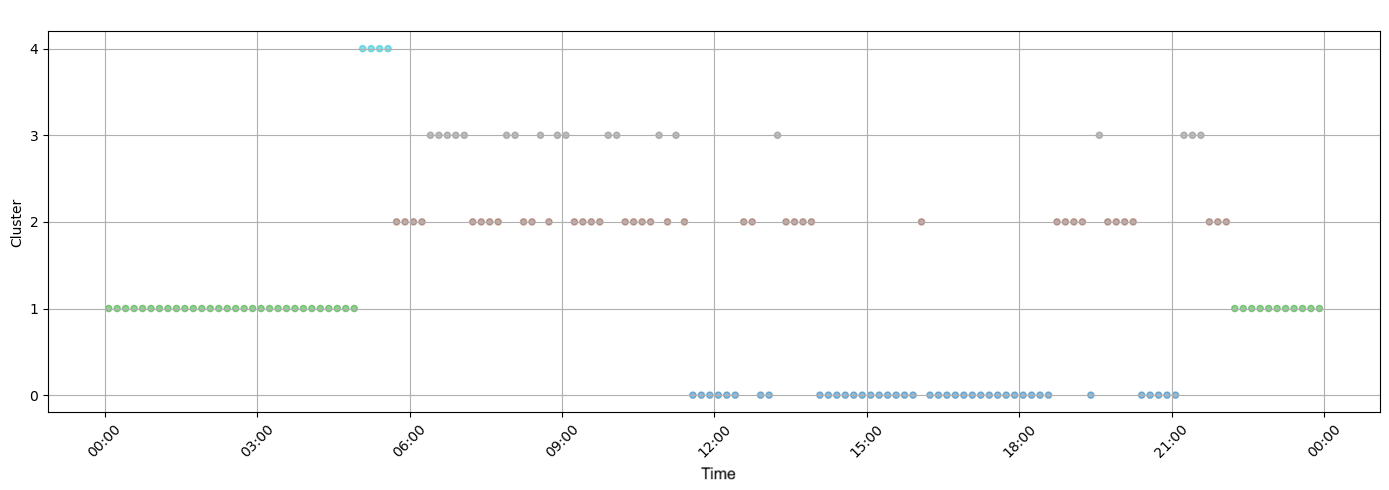
\includegraphics[width=0.95\textwidth]{figs/Figure_12.png}
\captionof{figure}{Daily temporal distribution of the Hierarchical Clustering clusters ($k=5$, 10-minute windows) throughout a workday.}
\label{fig:temporal_hier_janela}
\end{center}

The temporal distribution shows a more stable organization of the states, with relatively well-defined blocks throughout the workday. A coherent sequence is observed between nighttime rest, awakening, periods of activity and travel, the workday, and occasional episodes of greater physical effort. Compared with the model trained on minute-level data, temporal aggregation reduces alternation between clusters and favors a more continuous representation of physiological behavior. This result reinforces the positive effect of temporal windows on cluster interpretation, allowing Hierarchical Clustering to represent states that are more consistent and aligned with different moments of the daily routine.

\subsection{External Validation with Experimental Data}\label{sec:external_validation}

To complement the evaluation of the clustering models, an additional experiment was conducted using physiological data collected directly through a smartwatch in different everyday situations. The objective was to verify whether the physiological states previously identified from the training data were also consistently recognized in independent data not used during learning. Three distinct situations were considered: \textbf{physical activity}, including weightlifting and high-intensity cardiovascular exercise; \textbf{computer work}, representing a situation involving concentration and cognitive load; and \textbf{sleep}, corresponding to a prolonged rest period. The data were collected on April 24 and 25, 2026, covering approximately two hours of physical activity, two hours of computer work, and 5~h~46~min of sleep.

To ensure consistency between training and external validation, the experimental data were subjected to the same preprocessing \textit{pipeline} used to construct each model. Thus, the transformations specific to each configuration were applied, including missing-value handling, anomaly and \textit{outlier} detection and treatment, normalization and \textit{scaling}, categorical-variable encoding, and, for the GMM models, PCA transformation. After this processing, the data were entered into the four previously trained models: \textbf{GMM} with original data ($k=9$), \textbf{GMM} with 10-minute windows ($k=5$), \textbf{Hierarchical Clustering} with original data ($k=5$), and \textbf{Hierarchical Clustering} with 10-minute windows ($k=5$). Thus, the models were not refitted to the experimental data, allowing the generalization capacity of the previously obtained configurations to be assessed directly.

The evaluation was based on the physiological interpretation previously assigned to each \textit{cluster}. For each model, the \textit{clusters} considered compatible with each experimental activity were defined. For example, in the GMM with $k=9$, \textit{clusters} 0 and 5 were associated with deep sleep, \textit{clusters} 3, 4, and 8 with physical activity, and \textit{clusters} 2, 6, and 7 with work or concentration. Thus, a prediction belonging to any of the \textit{clusters} expected for a given activity was considered a correct classification, whereas a prediction outside this set was considered incorrect. This procedure transforms the unsupervised assignment of \textit{clusters} into a measure of agreement between the expected physiological state and the state identified by the model.

The results reveal important differences between the evaluated configurations. For the original data, the GMM achieved an \textit{accuracy} of 75.17\% for physical activity and 82.64\% for computer work, whereas \textit{accuracy} during sleep was 46.09\%. Hierarchical Clustering yielded values of 59.73\% for physical activity, 81.82\% for computer work, and 93.04\% for sleep. These results show that, although the GMM performed competitively in identifying physical activity and work, the hierarchical model had clearly superior ability to recognize the sleep period.

Figures~\ref{fig:external_gmm_pc}, \ref{fig:external_gmm_exercise}, and \ref{fig:external_gmm_sleep} present, respectively, the temporal distribution of the predictions obtained by the GMM with original data ($k=9$) during sleep, computer work, and physical activity. Green points represent predictions belonging to the \textit{clusters} considered compatible with the experimental activity, whereas red points correspond to predictions outside the expected \textit{clusters}. This representation makes it possible to observe not only the overall \textit{accuracy}, but also the temporal distribution of correct and incorrect predictions throughout each experimental period. For computer work, predictions are predominantly assigned to the \textit{cluster} associated with work or concentration, consistent with the \textit{accuracy} of 82.64\%. During physical activity, most predictions are concentrated in the \textit{clusters} associated with physical activity, although periods of classification into work- or concentration-related states occur. During sleep, despite the prolonged presence of predictions in \textit{cluster} 0, a considerable number of classifications occur in states not associated with deep sleep, which is consistent with the lower \textit{accuracy} observed for this condition.

\begin{center}
    \centering
  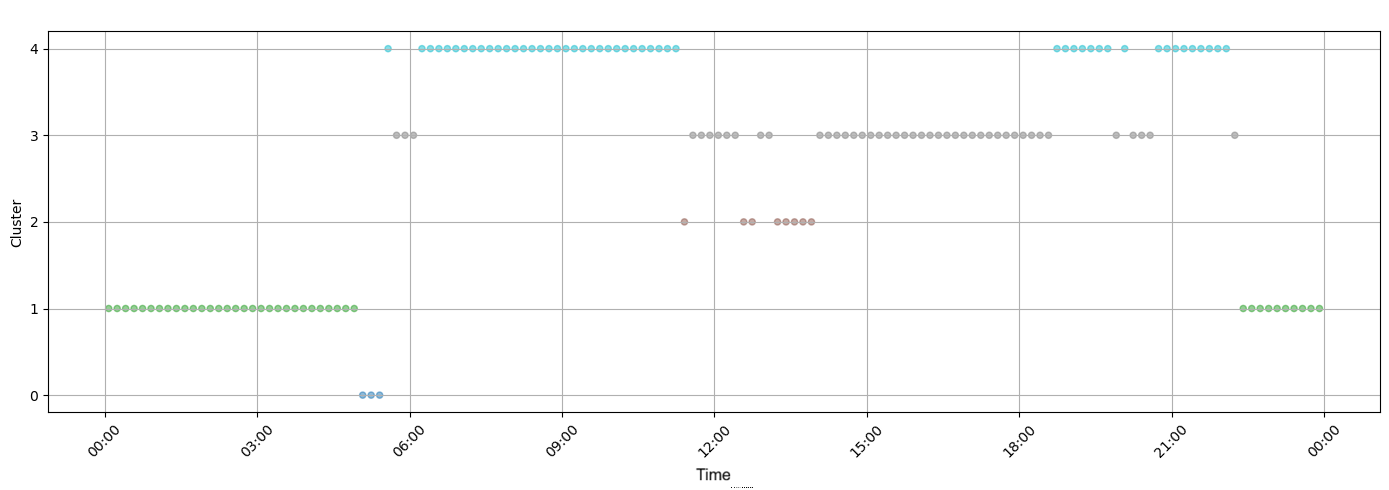
\includegraphics[width=0.95\textwidth]{figs/Figure_13.png}
    \captionof{figure}{Temporal distribution of GMM predictions ($k=9$) during computer work.}
    \label{fig:external_gmm_pc}
\end{center}

\begin{center}
    \centering
  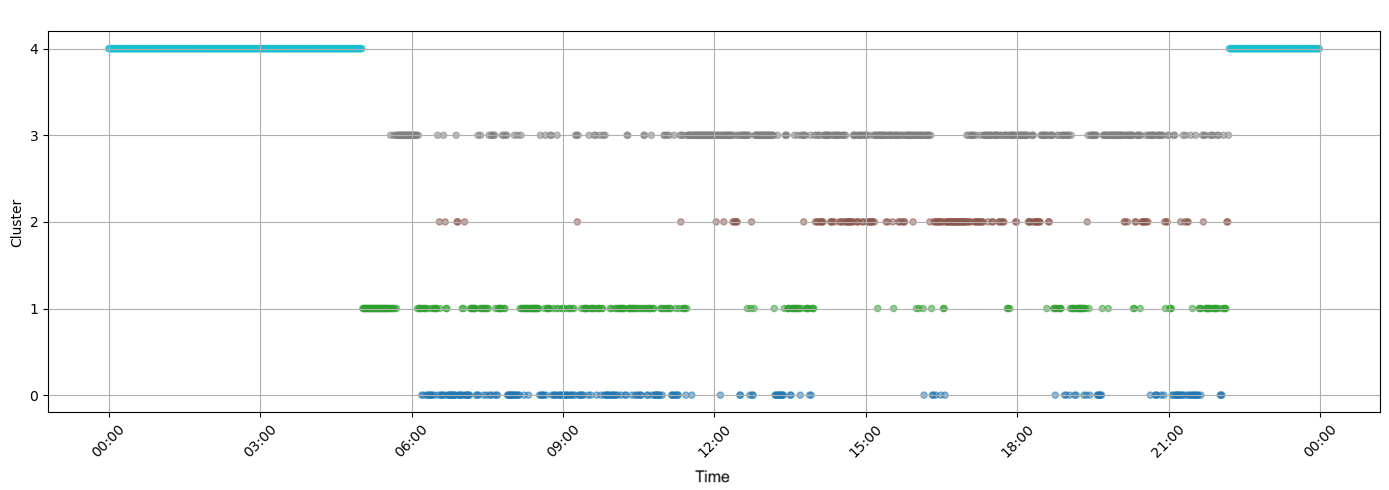
\includegraphics[width=0.95\textwidth]{figs/Figure_14.png}
    \captionof{figure}{Temporal distribution of GMM predictions ($k=9$) during physical activity.}
    \label{fig:external_gmm_exercise}
\end{center}

\begin{center}
    \centering
  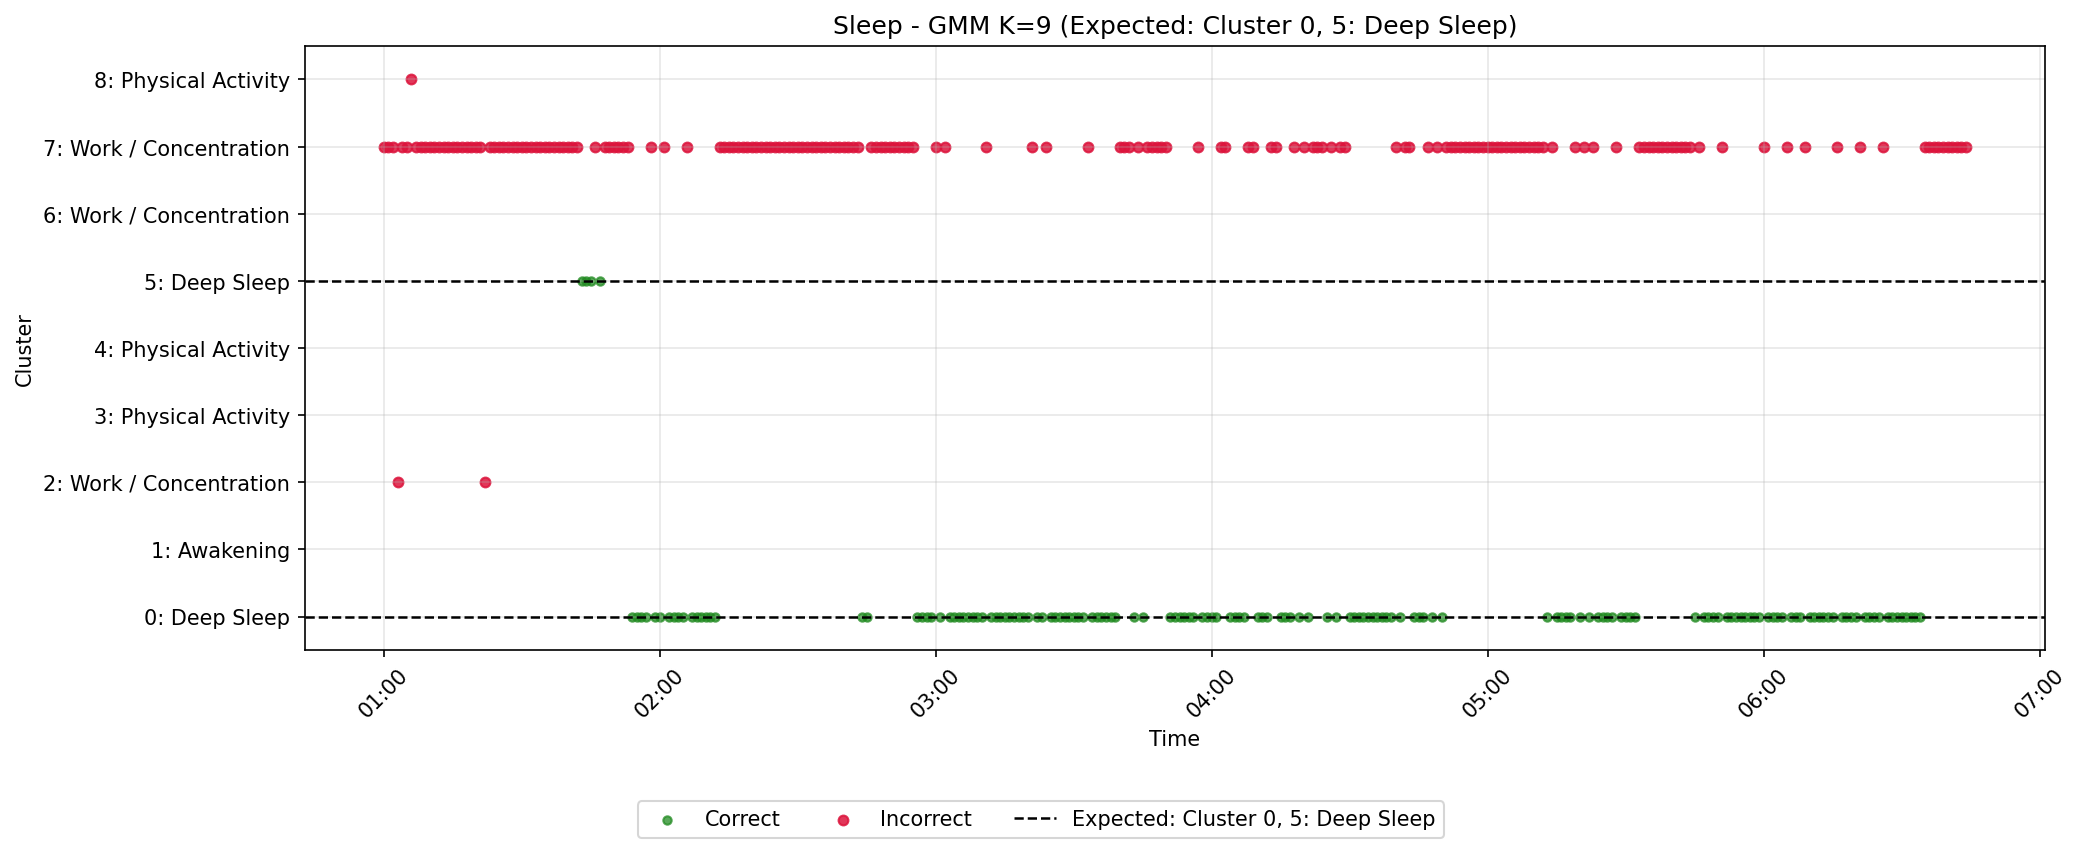
\includegraphics[width=0.95\textwidth]{figs/Figure_15.png}
    \captionof{figure}{Temporal distribution of GMM predictions ($k=9$) during the sleep period.}
    \label{fig:external_gmm_sleep}
\end{center}

For the models based on 10-minute temporal windows, the GMM achieved an \textit{accuracy} of 26.67\% for physical activity, 76.92\% for computer work, and 51.43\% for sleep. Hierarchical Clustering produced markedly different results: 0.00\% for physical activity, 23.08\% for computer work, and 100.00\% for sleep. These results indicate that temporal aggregation did not produce a uniform improvement in activity recognition. For sleep, the windowed representation clearly favored Hierarchical Clustering, which correctly classified all 35 evaluated windows. On the other hand, the same representation showed significant difficulties in identifying physical activity and computer work, particularly for the hierarchical model.

\begin{center}
\captionof{table}{Accuracy of external validation for the different model configurations.}
\label{tab:external_validation}
\small
\begin{tabular*}{.95\textwidth}{@{} p{.34\linewidth} p{.18\linewidth} p{.18\linewidth} p{.16\linewidth} @{}}
\toprule
\textbf{Model} & \textbf{Physical activity} & \textbf{Work/PC} & \textbf{Sleep} \\
\midrule
GMM ($k=9$) & 75,17\% & 82,64\% & 46,09\% \\
Hierarchical ($k=5$) & 59.73\% & 81.82\% & 93.04\% \\
GMM, windows ($k=5$) & 26.67\% & 76.92\% & 51.43\% \\
Hierarchical, windows ($k=5$) & 0.00\% & 23.08\% & 100.00\% \\
\bottomrule
\end{tabular*}
\end{center}

Taken together, this external validation shows that no single configuration provides the best performance in all physiological situations. The \textbf{GMM} with original data showed the most balanced behavior for physical activity and computer work, whereas \textbf{Hierarchical Clustering} with original data stood out in sleep identification. The 10-minute window representation further strengthened identification of the rest state in the hierarchical model, but significantly impaired discrimination of short-duration or highly variable activities, such as exercise and certain work situations. These results are particularly relevant because they demonstrate that clustering quality should not be assessed exclusively through internal metrics, but also through its ability to produce coherent physiological states when applied to independent and experimentally controlled data.


%%%%%%%%%%%%%%%%%%%%
% CONCLUSIONS AND FUTURE WORK
%%%%%%%%%%%%%%%%%%%%
\section{Conclusions and Future Work}\label{sec:conclusions}

This study evaluated two unsupervised learning approaches, the Gaussian Mixture Model (GMM) and Agglomerative Hierarchical Clustering, to identify physiological states from signals collected by an Empatica EmbracePlus wrist-worn wearable device. The analysis of the minute-level data and the data aggregated into 10-minute windows showed that the models can distinguish patterns associated with rest and sleep, daily activity, cognitive load, and physical effort, although the physiological meaning of the clusters depends on the algorithm and temporal resolution used.

The selection of the number of clusters benefited from the joint use of internal metrics, namely BIC, the Silhouette index, the elbow method, and dendrogram analysis. However, the results also showed that these metrics, considered in isolation, are not sufficient to select a final solution: physiological interpretability and temporal coherence of the clusters were necessary to avoid excessively fragmented or overly general solutions.

External validation confirmed that there is no optimal model for all the activities evaluated. Performance varied according to the physiological state and temporal representation. In general, the original data preserved information associated with dynamic activities more effectively, although this behavior was not uniform across the models. In contrast, temporal aggregation particularly favored Hierarchical Clustering in sleep identification, but did not constitute a general advantage for all activities. Thus, 10-minute windows may favor the representation of prolonged states, but may also attenuate short-duration or highly variable patterns.

Taken together, these results indicate that physiological clustering should not be evaluated exclusively through the Silhouette index or WCSS. Validation with independent and experimentally controlled data provides complementary evidence more directly related to the practical utility of the clusters, making it possible to verify whether the identified states retain their meaning when applied beyond the data used for training. The study therefore supports the potential of unsupervised approaches to characterize physiological states relevant to fatigue monitoring and future occupational-safety support systems, although it does not yet constitute sufficient validation for autonomous operational use.

The main limitation lies in the limited scope of the external validation, which covered three experimental situations and a restricted collection period. In future work, it will be important to evaluate these models on larger and more diverse datasets, including different workers, environmental conditions, tasks, and seasonal periods. The stability and latency of the predictions should also be studied prospectively in a potential integration with Human Digital Twin platforms, together with the possibility of adapting the models to other industrial contexts.

\section*{Acknowledgment}

This research was supported by the CRIARTE project, funded by the European Regional Development Fund (ERDF) through the COMPETE 2030 Programme, project number COMPETE2030-FEDER-01192200, and by national funds from the Portuguese Foundation for Science and Technology (FCT), under the R\&D Units Project Scope UID/00760/2025.

% Numbered list
% Use the style of numbering in square brackets.
% If nothing is used, default style will be taken.
%\begin{enumerate}[a)]
%\item 
%\item 
%\item 
%\end{enumerate}  

% Unnumbered list
%\begin{itemize}
%\item 
%\item 
%\item 
%\end{itemize}  

% Description list
%\begin{description}
%\item[]
%\item[] 
%\item[] 
%\end{description}  

% Uncomment and use as the case may be
%\begin{theorem} 
%\end{theorem}

% Uncomment and use as the case may be
%\begin{lemma} 
%\end{lemma}

%% The Appendices part is started with the command \appendix;
%% appendix sections are then done as normal sections
%% \appendix

% To print the credit authorship contribution details
\printcredits

%% Loading bibliography style file
%\bibliographystyle{model1-num-names}
\bibliographystyle{cas-model2-names}

% Loading bibliography database
\bibliography{cas-refs}

% Biography
%\bio{}
% Here goes the biography details.
%\endbio

%\bio{pic1}
% Here goes the biography details.
%\endbio

\end{document}

